\chapter{Objetivos y Descripci\'on de la Soluci\'on}

Nuestra meta en este documento es analizar la capa de servicios web de una aplicaci\'on, desde la definici\'on formal de dicha interfaz hasta la implementaci\'on herramientas y librer\'ias software que permitan el desarrollo de \textit{APIs} que combinen las tecnolog\'ias sem\'anticas con los principios arquitecturales web \textit{REST}, para ofrecer una alternativa pragm\'atica y viable a desarrolladores web que solucione las limitaciones de las que adolecen las t\'ecnicas actuales de desarrollo de \textit{APIs}.\\
Los principales componentes de este an\'alisis y que se desarrollar\'an en este documento, son los siguientes:\\

\begin{itemize}

\item \textbf{Modelo formal} de la capa de servicios web y agentes consumiendo dichos servicios, que constituye la interacci\'on b\'asica de cualquier \textit{API} de datos.

\item \textbf{Dise\~no de una soluci\'on arquitect\'onica} basada en los principios de arquitectura \textit{REST} que permita exponer datos enlazados en nuevas \textit{APIs} y servicios. Algunas de las caracter\'isticas con las que debe contar esta arquitectura pasan por la separaci\'on radical entre clientes y capa de servicio, el uso de la negociaci\'on de contenido para obtener la adecuada representaci\'on de los datos por parte del cliente, ser completamente agn\'ostica en cuanto al mecanismo  de almacenamiento del grafo de datos enlazados usado en la implementaci\'on final, utilizar el concepto de recurso web como la unidad fundamental de datos que son expuestos y agregados.

\item \textbf{Implementaci\'on componentes software} que permitan la f\'acil construcci\'on de aplicaciones clientes y servidores que consuman datos enlazados a trav\'es de la arquitectura para \textit{APIs} sem\'anticas anteriormente especificada. As\'i mismo tambi\'en se mostrar\'a como se pueden adaptar tecnolog\'ias  ampliamente usadas hoy en d\'ia para facilitar el almacenamiento de datos enlazados, de tal forma que puedan ser utilizadas como repositorios de datos para los recursos expuestos a trav\'es de la arquitectura para \textit{APIs} desarrollada.

\item \textbf{Ejemplos de aplicaci\'on} en la capa de cliente de tal modo que se puedan mostrar ejemplos pr\'acticos de como el uso de \textit{APIs} sem\'anticas y las tecnolog\'ias asociadas permiten facilitar el desarrollo de aplicaciones web centradas en datos, as\'i como ofrecer nuevas funcionalidades para los usuarios.

\end{itemize}

La meta \'ultima de este trabajo es aplicar dichas tecnolog\'ias y herramientas a la construcci\'on de una aplicaci\'on web social, completamente descentralizada, donde la interconexi\'on de diferentes servicios asociados a distintos usuarios, controlando en todo momento los datos que generan as\'i como su identidad web, permita replicar la funcionalidad de las aplicaciones sociales centralizadas y dif\'icilmente inter-operables disponibles hoy en d\'ia.

\section{Model Formal}

Como hemos visto en los apartados del estado del arte relacionados con la construcci\'on de servicios web sem\'anticos, existen diferentes propuestas, para a\~nadir una capa sem\'antica a las \textit{APIs} de servicios web \textit{REST} expuestas por diferentes aplicaciones, por ejemplo, \textit{hRESTS} \cite{hrests} o \textit{SA-REST} \cite{sarest}. Sin embargos, estas propuestas se centran en detalles t\'ecnicos como diferentes t\'ecnicas de marcado sem\'antico y vocabularios espec\'ificos para describir los componentes esenciales de lo que supone el modelo \textit{REST} de servicios web sin ofrecer un verdadero modelo formal que permita describir soluciones computacionales a diferentes problemas, mediante el uso de servicios web \textit{REST} y meta-datos sem\'anticos. Dicho modelo, deber\'ia ser capaz de permitir dicha descripci\'on y servir de base sobre la que construir los diferentes componentes tecnol\'ogicos necesarios para implementar la soluci\'on descrita.\\
En este cap\'itulo propondremos un posible modelo formal que puede ser utilizado para describir de forma gen\'erica cualquier computaci\'on basada en el uso de servicios web \textit{REST} sem\'anticos.\\
Nuestro modelo se basa en dos referentes te\'oricos b\'asicos dentro del \'area de la computaci\'on distribuida:

\begin{itemize}
\item El uso de espacios de tripletes \cite{fensel2004triple} como un caso particular, adaptado al modelo de datos \textit{RDF} de los espacios de tuplas \cite{bussler2005minimal}, mecanismo de comunicaci\'on entre procesos mediante una memoria asociativa propuesto por Gelernter en sus art\'iculos sobre el sistem Linda \cite{linda}.

\item El C\'alculo Pi \cite{pi_calculus} un tipo de c\'alculo de procesos, en el que los procesos se comunican unos con otros a trav\'es del intercambio de mensajes a trav\'es de canales con nombre identificativo. Dichos mensajes pueden a su vez incluir los identificadores de los canales, con lo que los procesos pueden acceder a canales con los que comunicarse con nuevos procesos simplemente recibi\'endolos en un mensaje, variando de esta forma din\'amicamente con el tiempo la topolog\'ia de la red de canales y procesos que llevan a cabo una determinada computaci\'on.
\end{itemize}

El uso de estas dos bases te\'oricas en nuestra propuesta de c\'alculo formal es debida a la identificaci\'on de los componentes principales de la computaci\'on mediante servicios \textit{REST} con los componentes b\'asicos de los modelos de espacios de tripletes y el C\'alculo Pi.\\

Esta identificaci\'on se basa en los siguientes supuestos:
\begin{itemize}

\item Un recurso \textit{REST} sem\'antico consiste en un conjunto de tripletes \textit{RDF} almacenados en en un repositorio accesible por los procesos participando en la computaci\'on. Un recurso \textit{REST} sem\'antico consiste en un espacio de tripletes.

\item El espacio de tripletes que constituye el recurso \textit{REST} sem\'antico es accesible a trav\'es de un \textit{URI} asociado que puede ser enlazado desde otros recursos relacionados. Los \textit{URIs} asociados a los recursos se pueden considerar pues canales con identificadores como los que se usan los procesos del C\'alculo Pi para intercambiar mensajes.

\item El espacio de tripletes que que contiene los tripletes \textit{RDF} del recurso puede ser manipulado mediante peticiones \textit{HTTP} sobre el \textit{URI} asociado al recurso, de acuerdo con la sem\'antica propia de la interfaz uniforme \textit{HTTP}. De este modo, la sem\'antica de la interfaz \textit{HTTP} se puede traducir a las operaciones b\'asicas del C\'alculo Pi y por \'ultimo a las operaciones elementales sobre un espacio de tripletes.

\end{itemize}

Ejemplos de entornos de servicios web que cumplen estos supuestos son, servicios web en los que se intercambian documento \textit{HTML} con anotaciones sem\'anticas insertadas usando el est\'andar \textit{RDFa} o \textit{APIs} de servicios web que permiten a acceder a grafos \textit{RDF} almacenados en un repositorio de tripletes a trav\'es de una interfaz \textit{HTTP} \textit{REST}.\\
En los siguientes apartados explicaremos pormenorizadamente los detalles que permiten la identificaci\'on de un recurso \textit{REST} sem\'antico tanto con un espacio de tripletes como con un proceso dentro del C\'alculo Pi y que forman la base de nuestra propuesta de c\'alculo de procesos para servicios web sem\'anticos.

\subsection{Recursos sem\'anticos y espacios de tripletes}

La base del c\'alculo es la manipulaci\'on de meta-datos sem\'anticos representados como tripletes \textit{RDF}. Los componentes de un triplete pueden consistir de \textit{URIs} o literales. Cualquier computaci\'on descrita en el c\'alculo consiste en la manipulaci\'on de tripletes almacenados en espacios de datos compartidos denominados espacios de tripletes \cite{fensel2004triple} por un conjunto de procesos distribuidos.\\
Este modelo de computaci\'on distribuida se conoce como comunicaci\'on generativa de acuerdo con la terminolog\'ia propia de los sistemas de espacios de tuplas como Linda \cite{linda}. En estos sistemas se describe un conjunto finito de operaciones sobre el espacio de tuplas. Estas operaciones se pueden adaptar para manipular tripletes almacenados en un espacio de tripletes:

\begin{itemize}
\item \textbf{Rd:} Operaci\'on que permite leer tripletes del espacio de tripletes sin eliminarlos del repositorio. 
\item \textbf{Rdb:} Versi\'on bloqueante de la operaci\'on rd.
\item \textbf{In:} Operaci\'on que permite leer tripletes del espacio de tripletes elimin\'andolos del repositorio al mismo tiempo.
\item \textbf{Inb:} Versi\'on bloquente de la operaci\'on in.
\item \textbf{Out:} Operaci\'on que permite insertar tripletes en el espacio de tripletes.
\item \textbf{Notify \cite{busi2000process}:} Operaci\'on que permite a los procesos recibir una notificaci\'on cuando otros procesos manipulan el espacio de tripletes de una determinada manera.
\item \textbf{Swap \cite{bessani2008depspace}:} Operaci\'on que combina lectura, borrado y escritura en una sola operaci\'on at\'omica sobre el espacio de tripletes.

\end{itemize}

Las operaciones definidas en el c\'aculo sobre espacios de tripletes aceptan como argumentos tanto conjuntos de tripletes ($v$), como patrones ($p$). La sem\'antica particular del mecanismo de definici\'on de patrones y su aplicaci\'on sobre el espacio de tripletes puede variar sin afectar a la sem\'antica del c\'alculo. En este documento supondremos un mecanismo basado en un subconjunto de \textit{SPARQL} consistente s\'olo en la aplicaci\'on de patrones b\'asicos de grafo (\textbf{BGP}) con sustituci\'on simple de nombres \cite{sparql}.\\
Un patr\'on recibido en una operaci\'on puede ser aplicado a un conjunto de tripletes $(< p,v >$) o a un espacio de tripletes ($< p,\theta >$), obteni\'endose como resultado una colecci\'on de substituciones para las variables del patr\'on. Aplicando estas substituciones al patr\'on el conjunto de tripletes que satisfacen dicho patr\'on es obtenido finalmente. El resultado de la aplicaci\'on del patr\'on puede ser el conjunto vac\'io, si ninguna substituci\'on es obtenida.\\
Una definici\'on exacta de la sintaxis y sem\'antica operacional del c\'alculo, se pueden encontrar en las tablas \ref{tabla1} y \ref{tabla2}.\\

\begin{table}
\vspace{2.4in}
\caption{Sintaxis formal del calculo relativa al espacio de tripletes y elementos b\'asicos.}
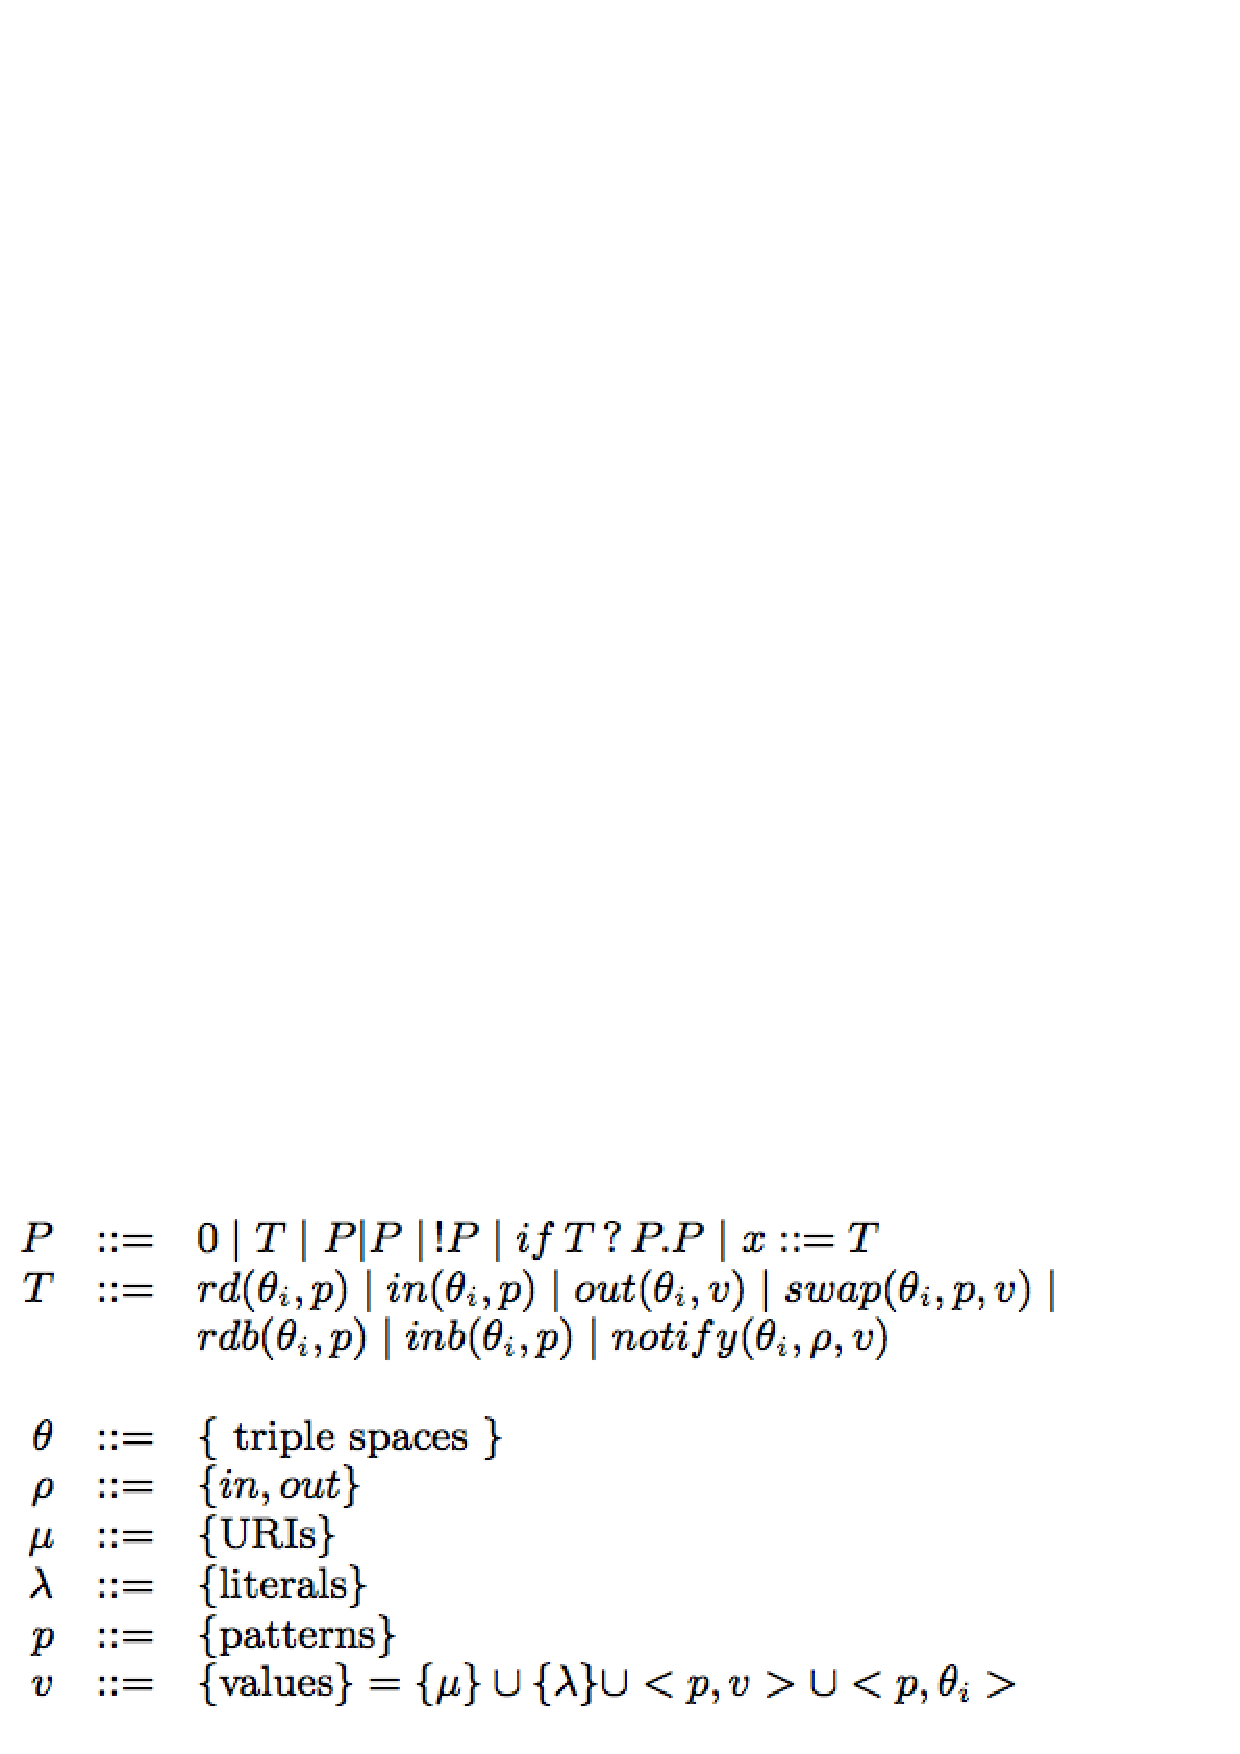
\includegraphics[width=0.8\textwidth]{tabla1}
\label{tabla1}
\end{table}


\begin{table}
\vspace{2.4in}
\caption{Sem\'antica operacional del calculo relativa al espacio de tripletes y operaciones b\'asicas.}
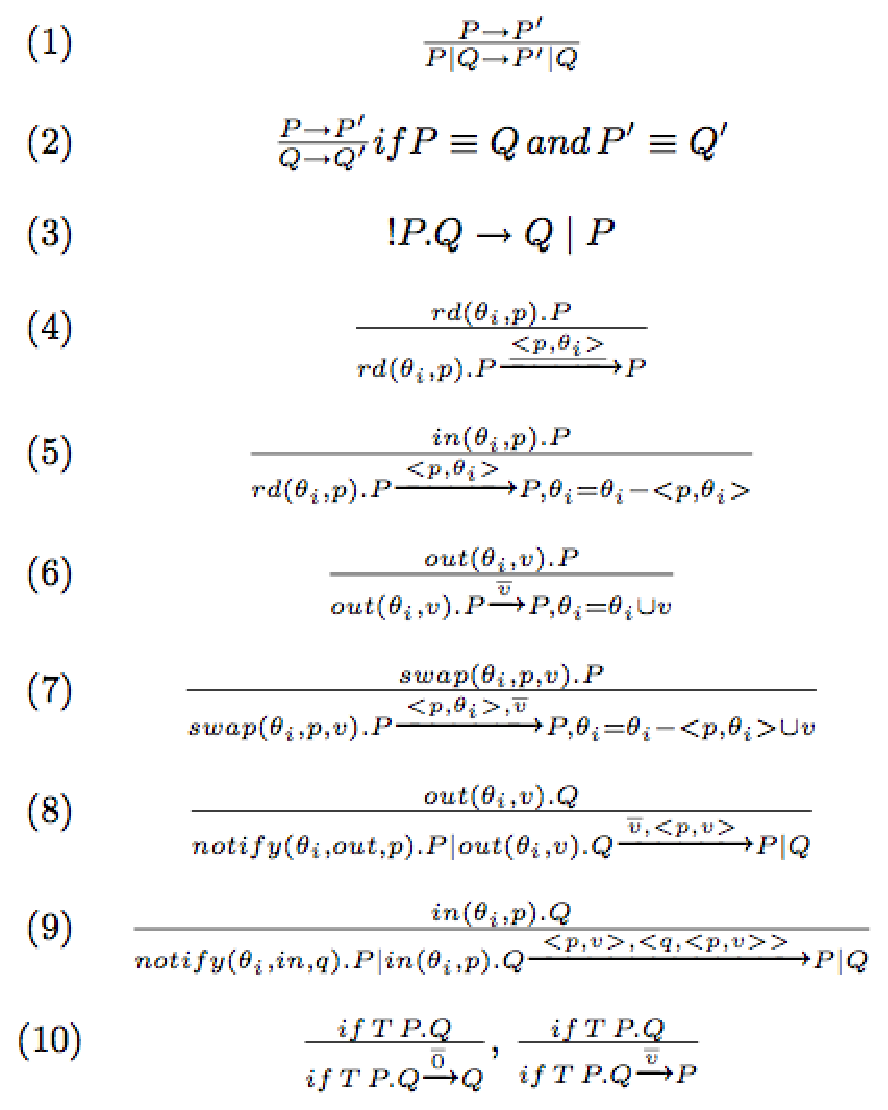
\includegraphics[width=0.8\textwidth]{tabla2}
\label{tabla2}
\end{table}

La sem\'antica operacional del c\'alculo para la sintaxis formal aqu\'i introducida sigue formalizaciones anteriores propuestas para otros sistemas de espacios de tuplas de tipo Linda \cite{linda}. En particular, hemos elegido una sem\'antica con ordenaci\'on para las operaciones sobre el espacio de tripletes. Como consecuencia, la emisi\'on y aplicaci\'on de mensajes se puede considerar como una \'unica operaci\'on at\'omica. Se puede demostrar que los sistemas de tipo Linda con semanticas con con ordenaci\'on son Turing completos \cite{busi2000expressiveness}.\\
La sem\'antica operacional descrita en la tabla \ref{tabla2}, define una relaci\'on ($\rightarrow$) para las operaciones como la m\'as simple interpretaci\'on satisfaciendo las reglas ($1$) – ($10$). De estas, las comprendidas entre la regla ($4$)  y la regla ($6$) definen las principales operaciones sobre espacios de tripletes as\'i como la reducci\'on de estas reglas modifican los tripletes almacenados en el espacio de tripletes.\\
La regla ($7$) muestra la sem\'antica de la operaci\'on swap como una combinaci\'on en un s\'olo paso de reducci\'on de la sem\'antica de las operaciones in y out. Por su parte, las reglas ($8$) y ($9$) definen las sem\'antica para la operaci\'on notify. Mostrando su relaci\'on con la operaci\'on in y out as\'i como el patr\'on pasado como argumento a la operaci\'on notify es aplicado a los tripletes insertados o eliminados por las operaciones in y out.\\

Como ya mencionamos, nuestra propuesta de c\'alculo se basa en la identificaci\'on de los elementos b\'asicos del modelo de servicios \textit{REST} con los axiomas formales introducidos en el modelo formal. Desde este punto de vista, las siguientes identidades entre c\'alculo y modelo \textit{REST} pueden ser establecidas:

\begin{itemize}

\item Un conjunto de tripletes en un espacio de tripletes puede ser identificado como un recurso \textit{HTTP}.
\item Un identificador del espacio de tripletes puede hacerse equivalente a un \textit{URI} asociado a un recurso \textit{HTTP}.
\item Las operaciones \textit{GET} del protocolo \textit{HTTP} son equivalentes a operaciones rd sobre el espacio de tripletes.
\item Las operaciones \textit{POST} del protocolo \textit{HTTP} son equivalentes a operaciones out sobre el espacio de tripletes.
\item Las operaciones \textit{PUT} del protocolo \textit{HTTP} son equivalentes a operaciones swap sobre el espacio de tripletes.
\item Las operaciones \textit{DELETE} del protocolo \textit{HTTP} son equivalentes a operaciones in sobre el espacio de tripletes.

\end{itemize}

\subsection{Recursos sem\'anticos y procesos en tiempo de ejecuci\'on}

Las sintaxis y sem\'antica introducidas en el c\'alculo en el punto anterior y relativas a la visi\'on de los recursos \textit{HTTP} sem\'anticos como tripletes almacenados en un espacio de tripletes no es suficiente para describir una computaci\'on completa involucrando servicios web \textit{REST} sem\'anticos.\\
En primer lugar, en las concepciones originales de los espacios de tripletes, el espacio de tripletes era global, \'unico y compartido. Sin embargo, para modelar recursos \textit{REST} sem\'anticos, es conveniente considerar cada recurso individual como un espacio de tripletes diferente e identificado por un \textit{URI}. Del mismo modo, estos espacios de tripletes no ser\'ian est\'aticos, sino que podr\'ian ser creados mediante operaciones \textit{HTTP} \textit{POST} y destruidos mediante operaciones \textit{HTTP} \textit{DELETE}. La identificaci\'on de las operaciones in y out con los m\'etodos \textit{HTTP} \textit{DELETE} y \textit{POST} ser\'ia pues incompleta, ya que tendr\'ian como objeto tripletes individuales y no el conjunto del espacio de tripletes. El formalismo puede ser extendido \cite{simperl2007coordination} a\~nadiendo nuevas operaciones tanto sobre espacios de tripletes como sobre tripletes individuales. Teniendo en cuenta estas extensiones, los espacios de tripletes podr\'ian ser concebidos como procesos en el c\'alculo que pueden ser creados, recibir mensajes de otros procesos y terminar su ejecuci\'on.\\
Otra importante identidad entre servicios \textit{REST} y espacios de tripletes introducida ha sido la capacidad de asociar un \textit{URI} a un espacio de tripletes. De este modo, los procesos pueden ganar acceso a los tripletes de un recurso almacenados en un espacio de tripletes a trav\'es de los \textit{URIs} codificados en sus componentes. Desde este punto de vista, los espacios de tripletes pueden ser considerados no s\'olo procesos din\'amicos, sino como procesos m\'obiles tal y como los descritos en el C\'alculo Pi, ya que estos procesos podr\'ian coordinarse a trav\'es de canales con nombre (\textit{URI}) que se intercambiar\'ian dentro de los componentes incluidos en los mensajes (tripletes) enviados y recibidos por los procesos.\\
En las tablas \ref{tabla1} y \ref{tabla2} se definen la sintaxis y sem\'antica operacional que permite describir los espacios de tripletes como procesos din\'amicos mediante la definici\'on de la composici\'on paralela de procesos ($1$) as\'i como la congruencia estructural de procesos ($2$) \cite{pi_calculus}. Por su parte ($3$) define el proceso de creaci\'on de un nuevo proceso y por \'ultimo ($10$) define un tipo sencillo de ejecuci\'on condicional.\\
Adem\'as de estas primitivas para la creaci\'on y composici\'on de procesos, el c\'alculo debe ser extendido con nuevas operaciones, como las mostradas en la tabla \ref{tabla3}, que corresponden a variaciones de las operaciones descritas en el C\'alculo Pi Poli\'adico \cite{polyadic_pi}.\\

\begin{table}
\vspace{2.4in}
\caption{Sem\'antica operacional del c\'alculo relativa a la comunicaci\'on entre procesos.}
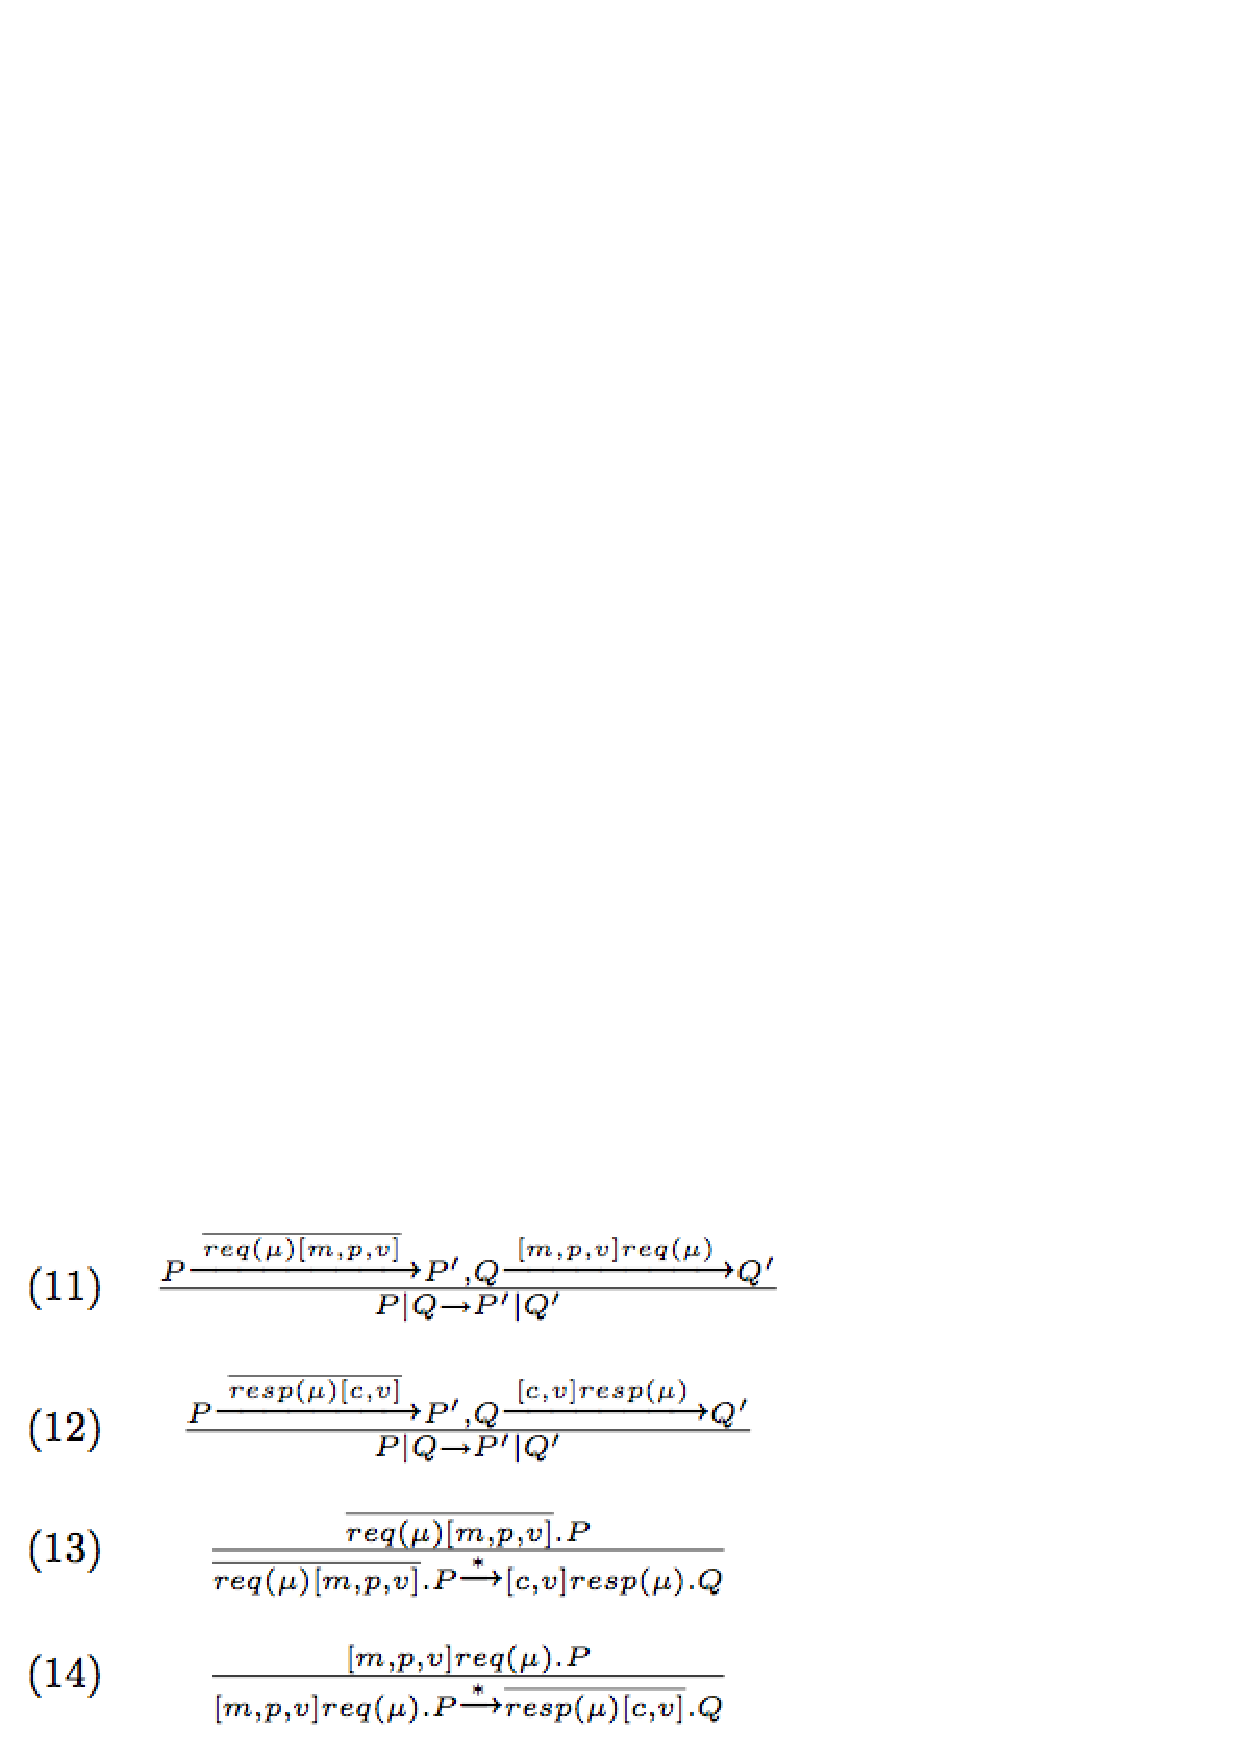
\includegraphics[width=0.8\textwidth]{tabla3}
\label{tabla3}
\end{table}

En dichas operaciones, los mensajes pueden ser enviados a trav\'es canales con nombre representados como \textit{URIs} ($\mu$). Los mensajes pueden ser de dos tipos, peticiones ($req$) o respuestas ($resp$) y los procesos pueden enviar y recibir ambos tipos de mensajes. A su vez, los mensajes se componen de un m\'etodo ($m$), un patr\'on ($p$) y un valor ($v$) en el caso de las peticiones y de un valor ($v$) y un c\'odigo ($c$) en el caso de las respuestas. Adicionalmente, tambi\'en se define una operaci\'on para introducir un nuevo identificador (\textit{URI}) en la computaci\'on. ($new\, \mu\, in\,P$).\\
La sem\'antica operacional para estas operaciones se introduce en la tabla \ref{tabla3} de acuerdo con la sem\'antica definida en el C\'alculo Pi Poli\'adico. Las reglas ($11$) y ($12$) son una adaptaci\'on a la sintaxis de nuestro c\'alculo de la regla de comunicaci\'on del C\'alculo Pi, mostrando la reacci\'on entre procesos enviando y recibiendo mensajes. Las reglas ($13$) y ($14$), imponen restricciones sobre el orden en que peticiones y respuestas deben ser intercambiados. Seg\'un la sem\'antica definida, sin un proceso env\'ia un mensaje con una petici\'on a un proceso, debe esperar un mensaje con una respuesta  tras un n\'umero finito de reducciones a trav\'es del mismo \textit{URI}. De modo sim\'etrico, si un proceso recibe una petici\'on a trav\'es de un \textit{URI} debe enviar una respuesta tras un cierto n\'umero de reducciones.\\

Esta sem\'antica permite modelar de una forma m\'as \'util en el c\'alculo las peticiones \textit{HTTP} a recursos \textit{REST} sem\'anticos como mensajes de petici\'on enviados a procesos a trav\'es de canales definidos como \textit{URIs} a recursos \textit{REST}. Estos mensajes consisten en un m\'etodo m\'as un patr\'on o tripletes y la respuestas vendr\'ian dadas por un codigo de respuesta m\'as un conjunto de tripletes. Nuevos recursos \textit{REST} sem\'anticos podr\'ian ser creados como resultado de peticiones POST asociados a nuevos \textit{URIs} introducidos en la computaci\'on y su ejecuci\'on podr\'ia terminar como resultado de una petici\'on DELETE. El sistema compuesto por estos recursos \textit{REST} sem\'anticos ser\'ia un c\'alculo de procesos m\'obiles dado que en los mensajes de respuesta provenientes de un recurso, podr\'ian encontrarse \textit{URIs} asociados a diferentes recursos.

\subsection{Modelado de recursos \textit{REST} sem\'anticos}

En las dos secciones previas, hemos introducido la notaci\'on y la sem\'antica de nuestro c\'alculo que permiten la descripci\'on de los recursos \textit{REST} sem\'anticos usando dos formalismos diferentes, los espacios de tripletes y el c\'alculo de procesos m\'oviles. Ambos mecanismos son complementarios siendo cada uno m\'as adecuado para la descripci\'on de diferentes aspectos de la computaci\'on con recursos \textit{REST} sem\'anticos. Los espacios de tripletes ofrecen una excelente descripci\'on de los recursos \textit{REST} sem\'anticos como repositorios est\'aticos de datos sem\'anticos, usando operaciones sobre los datos sem\'anticos como el principal mecanismo de coordinaci\'on entre los procesos manipulando dichos repositorios. De modo similar, el c\'alculo de procesos es adecuado para describir los aspectos din\'amicos del  protocolo \textit{HTTP}, como el mecanismo de paso de mensajes a trav\'es de canales con nombres, asociados a \textit{URIs}, entre procesos agentes y procesos que constituyen los recursos \textit{REST} sem\'anticos.\\
En esta secci\'on, una formalizaci\'on final del concepto de recurso \textit{REST} sem\'antico, que combina aspectos de ambos formalismos ser\'a llevada a cabo, usando para ello la sintaxis y la sem\'antica introducidas en las secciones anteriores.\\

Las principales caracter\'isticas de esta formalizaci\'on de la computaci\'on basada en recursos \textit{REST} sem\'anticos se enumeran a continuaci\'on:\\

\begin{itemize}
\item Cualquier computaci\'on es llevada a cabo por procesos distribuidos: agentes y recursos.
\item Cualquier proceso tiene un n\'umero de espacios de tripletes asociados que pueden ser manipulados por las operaciones sobre espacios de tripletes introducidas en la secci\'on 3.1.1.
\item Un cierto n\'umero de procesos compartiendo el acceso al mismo espacio de tripletes se pueden agrupar en una localizaci\'on computacional. Una aplicaci\'on web compuesta de multiples recursos web es un ejemplo de localizaci\'on computacional. Un navegador web ser\'ia otro ejemplo de localizaci\'on computacional compuesta \'unicamente de procesos agente.
\item Los procesos recurso tienen al menos un canal con nombre asociado (\textit{URI}) por el que pueden recibir mensajes de tipo petici\'on (req) enviados por otros procesos.
\item Los procesos agente no tienen un canal con nombre asociado (\textit{URI}), por lo que no pueden recibir mensajes de tipo petici\'on, pero pueden enviar mensajes de tipo petici\'on y recibir respuesta (resp) a procesos de tipo recurso a trav\'es de las \textit{URIs} almacenadas en sus espacios de tripletes.
\item La coordinaci\'on entre los procesos dentro de la misma localizaci\'on de computaci\'on se basa en las operaciones y sem\'antica definidas en el c\'alculo para las operaciones sobre espacios de tripletes.
\item Los canales con nombres (\textit{URIs}) pueden ser intercambiados a trav\'es de mensajes de petici\'on y respuesta y almacenados en espacios de tripletes como parte de los componentes de los tripletes.
\item La \'unica coordinaci\'on posible entre procesos en diferentes localizaciones de computaci\'on se basa en el paso de mensajes petici\'on y respuesta a trav\'es de canales con nombres (\textit{URIs}). Los identificadores de los espacios de tripletes no pueden ser intercambiados a trav\'es de mensajes petici\'on y respuesta.
\end{itemize}

Usando este modelo, una posible formalizaci\'on param\'etrica de un proceso sem\'antico \textit{REST} $S_{REST}(\theta,\mu)$, con un espacio de tripletes asociado ($\theta$), identificado por un \textit{URI} ($\mu$)  y que sigue la sem\'antica de la interfaz homog\'enea \textit{REST}, se muestra en la Tabla \ref{tabla4}.\\

\begin{table}
\vspace{2.4in}
\caption{Descripci\'on param\'etrica de un recurso \textit{REST} sem\'antico simple.}
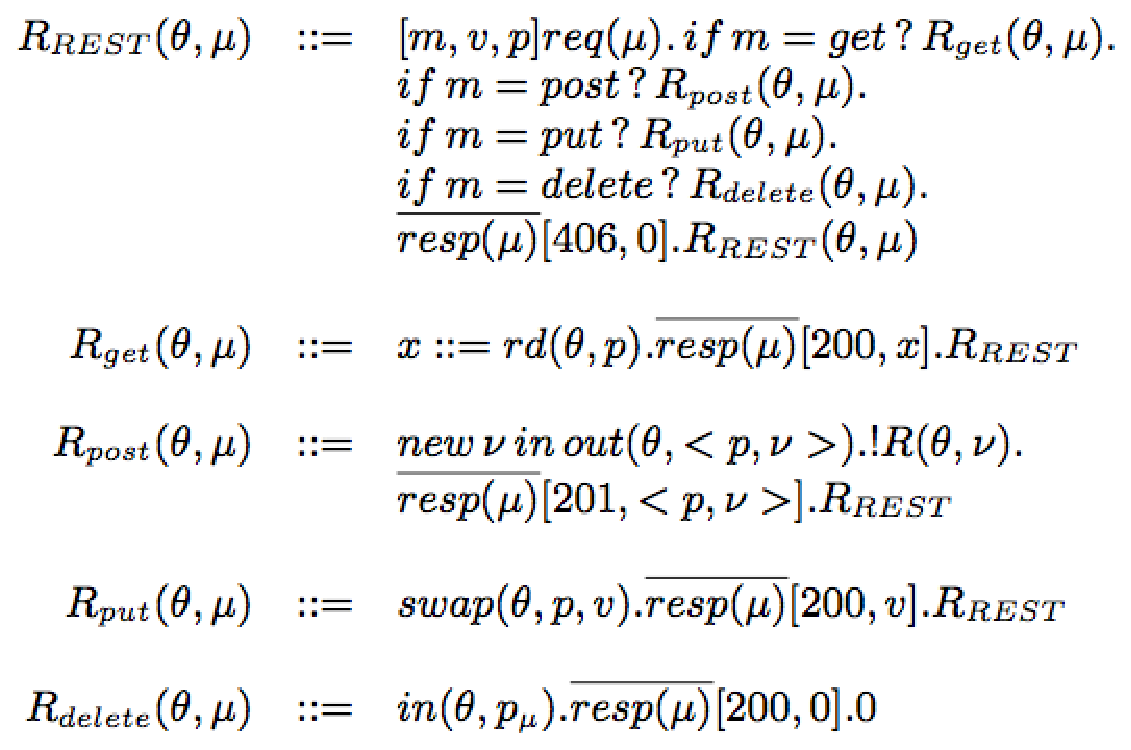
\includegraphics[width=0.8\textwidth]{tabla4}
\label{tabla4}
\end{table}


Seg\'un esta descripci\'on, el proceso recurso recibe espera un mensaje de tipo petici\'on y comprueba el tipo de la operaci\'on del mensaje.
Si es una petici\'on de tipo \textit{GET} incluyendo un patr\'on $p$, utiliza una operaci\'on sobre el espacio de tripletes $rd$ para leer sin extraer los tripletes que satisfagan el patr\'on y enviarlos a trav\'es de su \textit{URI} asociado al proceso que realiz\'o la petici\'on a trav\'es de un mensaje de tipo respuesta.\\
Si la petici\'on es de tipo \textit{POST}, incluyendo un patr\'on p con una \'unica variable, el proceso genera un nuevo \textit{URI} $\mu$ y lo aplica al patr\'on para obtener un nuevo conjunto de tripletes que escribe en su espacio de tripletes asociado $\theta$. Por \'ultimo un nuevo proceso recurso para los tripletes, espacio de tripletes y \textit{URI} asociada es iniciado por el proceso antes generar el mensaje respuesta al proceso que inici\'o la petici\'on.\\
Las peticiones \textit{PUT} son definidas a trav\'es de una operaci\'on \textit{swap} que aplica el patr\'on y nuevos valores enviados por un proceso en el mensaje de petici\'on. Las peticiones \textit{DELETE} por su parte, suponen la finalizaci\'on de la ejecuci\'on del proceso y el borrado del espacio de tripletes asociado de todos los tripletes asociados al \textit{URI} identificador del recurso.\\
La Figura \ref{figura1} muestra una representaci\'on gr\'afica de un posible modelo de ejecuci\'on de computaci\'on sem\'antica. Dicho modelo se compone de tres dominios que constituyen cada uno una localizaci\'on de computaci\'on independiente con su espacio de tripletes.\\

\begin{figure}
\vspace{2.4in}
\caption{Ejemplo de computaci\'on \textit{REST} sem\'antica.}
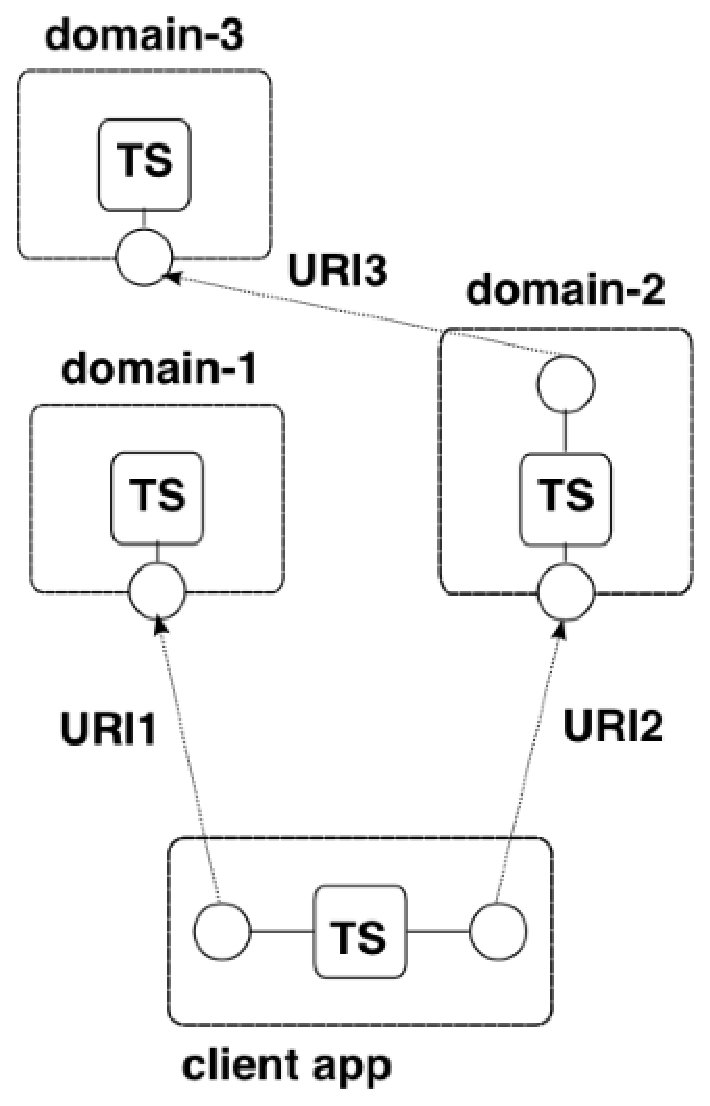
\includegraphics[width=0.5\textwidth]{figura1}
\label{figura1}
\end{figure}

Cada uno de ellos da soporte a un proceso recurso identificado por los \textit{URIs} 1, 2 y 3. Adem\'as, la localizaci\'on de computaci\'on constituida por el \textit{dominio-2} incluye tambi\'en un proceso agente que se puede comunicar con el servicio en el \textit{dominio-3} a trav\'es del \textit{URI} 3 almacenado en el espacio de tripletes presente en el \textit{dominio-2}. La figura tambi\'en muestra una localizaci\'on de computaci\'on adicional, que modela una aplicaci\'on web que contiene su propio espacio de tripletes y dos procesos agente. Dichos procesos agente pueden enviar mensajes de petici\'on a los servicios en los dominios 1 y 2 a trav\'es de las \textit{URIs} 1 y 2 almacenadas en el espacio de tripletes de la aplicaci\'on cliente. Por su parte el proceso recurso y el proceso agente localizado en el dominio-2 pueden coordinarse a trav\'es de operaciones sobre el espacio de tripletes del dominio,  por ejemplo a trav\'es de una operaci\'on notify, de tal modo que si el proceso recurso recibe un determinado mensaje de petici\'on, esto desencadene una notificaci\'on en el cliente para que pueda realizar una operaci\'on como reacci\'on, por ejemplo, enviar un mensaje de petici\'on al proceso recurso en el \textit{dominio-3}.

\section{Modelo arquitect\'onico}

En la secci\'on previa, se ha introducido un modelo formal que puede ser empleado para describir rigurosamente una computaci\'on basada en recursos \textit{REST} sem\'anticos.
Sin embargo, para transformar este modelo te\'orico en una implementaci\'on concreta de la soluci\'on, es necesario contar con un modelo de arquitectura software que sea consistente con las primitivas formales del c\'alculo descrito, definiendo al mismo tiempo las tecnolog\'ias y principales componentes con los que debe contar un sistema software que pretenda transformar dicho modelo formal en c\'odigo ejecutable.\\
En esta secci\'on describiremos este modelo arquitect\'onico, mediante la presentaci\'on de una ontolog\'ia \textit{RDF Schema} (\textit{RDFS}) que describe un modelo de servicios web que pueden dar soporte a las operaciones te\'oricas del c\'alculo de recursos \textit{REST} sem\'anticos discutido anteriormente y que sigue, al mismo tiempo, los principios arquitect\'onicos propuestos por la comunidad de Datos Enlazados Abiertos. Cualquier implementaci\'on de la arquitectura de servicios web \textit{REST} sem\'anticos que proponemos deber\'ia ser capaz de procesar autom\'aticamente una descripci\'on de una \textit{API} en los t\'erminos de la ontolog\'ia \textit{RDF} que proponemos y trasformarla en una serie de procesos software en tiempo de ejecuci\'on que ofrezcan los servicios especificados en dicha descripci\'on.\\
Los \'unicos componentes software que se presuponen es alg\'un tipo de adaptador \textit{HTTP} capaz de recibir en una interfaz de red peticiones en este protocolo, y un repositorio de grafos \textit{RDF} que soporte el lenguaje de consultas \textit{SPARQL 1.1 Update}. Esta versi\'on del lenguaje \textit{SPARQL} incluye no solo operaciones para recuperar informaci\'on desde el grafo \textit{RDF}, sino tambi\'en para modificar y eliminar tripletes del grafo.
El modelo arquitect\'onico de servicios web \textit{REST} sem\'anticos que vamos a describir, cumple con los siguientes requisitos fundamentales:

\begin{itemize}
\item Debe ser una alternativa viable para el desarrollo de \textit{APIs} de servicios web para el tipo de aplicaciones web que se desarrollan en la actualidad. A la hora de introducir nuevas tecnolog\'ias o conceptos, debe intentar hacerlo de una manera que resulte lo m\'as familiar posible para los desarrolladores web no familiarizados con las tecnolog\'ias estandarizadas por la comunidad Web Sem\'antica y Datos Enlazados Abiertos.
\item Debe permitir llevar a cabo una implementaci\'on software del c\'alculo formal de recursos \textit{REST} sem\'antico propuesto en la secci\'on previa de este documento.
\item Debe cumplir con los principios arquitecturales \textit{REST} y las recomendaciones de dise\~no originadas en la comunidad de Datos Enlazados Abiertos.
\item Debe dar soporte, no solo a la recuperaci\'on de datos, sino tambi\'en a la creaci\'on, actualizaci\'on y eliminaci\'on de recursos.
\item Debe intentar, dentro lo posible, reutilizar el trabajo y los vocabularios ya existentes dentro de la comunidad de Datos Enlazados Abiertos.
\end{itemize}

Dentro de las posible alternativas para la construcci\'on de una \textit{API} de servicios web para el acceso a grafos \textit{RDF} que mencionamos en apartados previos de este documento, la \textit{API} que vamos a describir se basa en el intercambio de grafos \textit{RDF} a trav\'es del protocolo \textit{HTTP}, tal y como establece la propuesta de recomendaci\'on de la \textit{W3C} para un  Protocolo \textit{SPARQL} \textit{HTTP} Uniforme para la Gesti\'on de Grafos \textit{RDF} \cite{ogbuji2011sparql}. Usando este protocolo, los recursos de informaci\'on en el servicio pueden ser descritos como tripletes almacenados en un \textit{grafo con nombre}. Esta concepci\'on de los recursos expuestos en la \textit{API} tambi\'en coincide con el concepto de recurso \textit{REST} sem\'antico descrito en el c\'alculo formal de recursos \textit{REST} sem\'anticos descrito anteriormente en este documento, donde  los tripletes de cada \textit{grafo con nombre} ser\'ian equivalentes al espacio de tripletes que respalda al proceso del c\'alculo que ofrece la funcionalidad \textit{REST} b\'asica y la \textit{URI} del \textit{grafo con nombre} har\'ia las veces del canal con nombre por el que los procesos agentes tendr\'ian acceso a los tripletes del recurso.
El uso de grafos con nombre como base para la definici\'on de recurso en la \textit{API} ofrece un nivel de granularidad similar al de otras \textit{APIs} \textit{REST} \cite{wilde2009restful}.\\
De forma adicional, introduciremos algunas caracter\'isticas convenientes que normalmente pueden encontrarse en \textit{APIs} basadas en entidades atributo-valor, como la propuesta LD-API \cite{ld_api} con el fin de facilitar el uso de la \textit{API} a clientes web con restricciones, como navegadores web.

\subsection{Declaraci\'on de recursos enlazados}

En la tabla \ref{tabla5} se encuentra la descripci\'on \textit{RDF} de un ejemplo de servicio web \textit{REST} sem\'antico, que se almacenar\'a en una base de datos relacional, de acuerdo con el modelo de servicio web que proponemos.\\

\begin{table}
\vspace{2.4in}
\caption{Descripci\'on \textit{RDF} de un servicio \textit{REST} sem\'antico.}
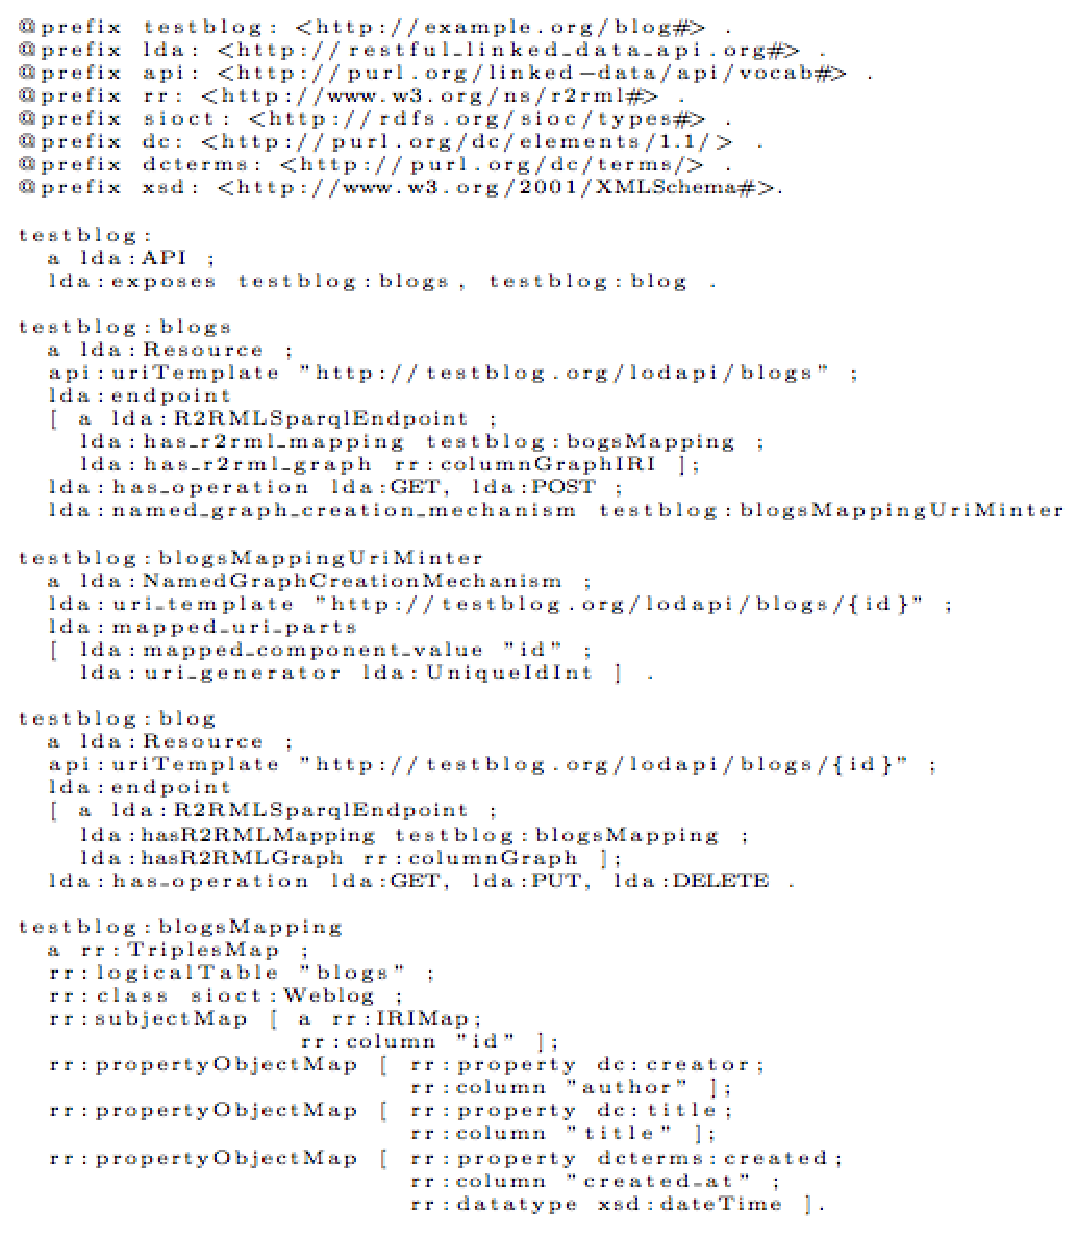
\includegraphics[width=0.8\textwidth]{tabla5}
\label{tabla5}
\end{table}

Esta descripci\'on describe dos aspectos b\'asicos del modelo de servicio:

\begin{itemize}
\item C\'omo se expone un conjunto de tripletes \textit{RDF} como un recurso \textit{REST} a trav\'es de la interfaz uniforme \textit{HTTP}.
\item C\'omo se transforman las peticiones \textit{HTTP} en consultas \textit{SPARQL} que cumplen con la sem\'antica que lo principios arquitect\'onicos \textit{REST} asignan a las operaciones \textit{GET}, \textit{POST}, \textit{PUT} y \textit{DELETE} del protocolo \textit{HTTP}.
\end{itemize}

Distintos elementos del vocabulario propuesto permite especificar los componentes de estos dos aspectos b\'asicos del modelo de servicio.\\
En el caso de la asociaci\'on entre el servicio y la interfaz \textit{HTTP}, el vocabulario ofrece las siguientes propiedades:

\begin{itemize}

\item \textbf{\textit{uriTemplate}:} Un patr\'on para un \textit{URI} que designa a un conjunto de grafos con nombre que podr\'an ser accedidos mediante operaciones \textit{HTTP}.  Esta propiedad de la ontolog\'ia se ha reutilizado de la especificaci\'on de LD-API, as\'i como la sem\'antica del proceso de validaci\'on de un \textit{URI} con un patr\'on \textit{URI} como el identifica esta propiedad.
\item \textbf{\textit{has\_operation}:} Asocia al recurso una collecci\'on de operaciones \textit{HTTP} que ser\'an v\'alidas a la hora de acceder a los datos almacenados en el \textit{grafo con nombre} expuesto como un recurso. \textit{lda:GET}, \textit{lda:PUT}, \textit{lda:POST} y \textit{lda:DELETE} son posible operaciones v\'alidas para esta propiedad. Estas operaciones deber\'an ser interpretadas por cualquier implementaci\'on de la arquitectura de acuerdo con lo acordado en la propuesta de recomendaci\'on sobre el Protocolo \textit{SPARQL} \textit{HTTP} Uniforme para la Gesti\'on de Grafos \textit{RDF}. En el siguiente apartado de este documento definiremos la sem\'antica para cada una de las operaciones anteriores como determinadas consultas \textit{SPARQL} 1.1/Update, compatibles con la sem\'antica de la interfaz uniforme \textit{HTTP}, tal y como se estableci\'o en el c\'alculo formal para recursos \textit{REST} sem\'anticos descrito en el cap\'itulo anterior de este documento.

\end{itemize}

El segundo aspecto del modelo servicio, la forma en que los datos sem\'anticos del recurso son almacenados en un repositorio de grafos \textit{RDF}/\textit{SPARQL}, viene dado por las siguientes propiedades:

\begin{itemize}
\item \textbf{\textit{endpoint}:} El repositorio \textit{RDF} en el que se almacenaran los conjuntos de tripletes \textit{RDF} que dan soporte a la informaci\'on de los diferentes recursos expuestos por la \textit{API}. Este repositorio debe ser capaz de soportar el conjunto de especificaciones \textit{SPARQL 1.1 Update}.
\item \textbf{\textit{named\_graph\_creation\_mechanism}:} Esta propiedad describe como nuevos grafos con nombre ser\'an generados cuando nuevos recursos necesiten ser creados. El mecanismo debe especificar un patr\'on de \textit{URI} para el nuevo \textit{grafo con nombre} as\'i como las partes del patr\'on que ser\'an generados. Dos mecanismos est\'an definidos en nuestro modelo de servicio: \textit{lda:UniqueIdInt} y \textit{lda:UUID}. El primero de ellos genera un nuevo entero \'unico mientras que el segundo genera un nuevo identificador universal \'unico \textit{UUID}.
\end{itemize}

\subsection{Modelo de Procesamiento del Servicio}

Las implementaciones software del modelo aq\'ii propuesto deben aceptar peticiones \textit{HTTP} y procesarlas en un esquema de tres etapas como el siguiente:\

\begin{itemize}
\item Traducci\'on de la petici\'on \textit{HTTP} a una petici\'on \textit{SPARQL}.
\item Generaci\'on de nuevos identificadores para grafos con nombre, si es necesario, y ejecuci\'on de la consulta \textit{SPARQL} en el repositorio de grafos \textit{RDF}.
\item Serializaci\'on del grafo \textit{RDF} resultante como en la representaci\'on acordada entre cliente y servidor mediante el proceso de negociaci\'on de contenido descrito en el protocolo \textit{HTTP}.
\end{itemize}

En la siguientes secciones analizaremos como se puede transformar cada tipo de operaci\'on \textit{HTTP} en consultas \textit{SPARQL} sobre un repositorio de grafos \textit{RDF} de manera que se conserve la sem\'antica que el protocolo \textit{HTTP}.

\subsubsection{Peticiones \textit{GET}}

Las peticiones  \textit{HTTP} \textit{GET} sobre un determinado \textit{URI} que identifica a un \textit{grafo con nombre} en el repositorio de grafos \textit{RDF}, se transforman en peticiones \textit{CONSTRUCT} \textit{SPARQL} que recuperan todos los tripletes almacenados en dicho \textit{grafo con nombre}.\\
La sintaxis de la consulta \textit{CONSTRUCT} \textit{SPARQL} se muestra en la tabla \ref{tabla6}.\\

\begin{table}
\vspace{2.4in}
\caption{Consulta \textit{SPARQL} para una peticion \textit{HTTP} \textit{GET}.}
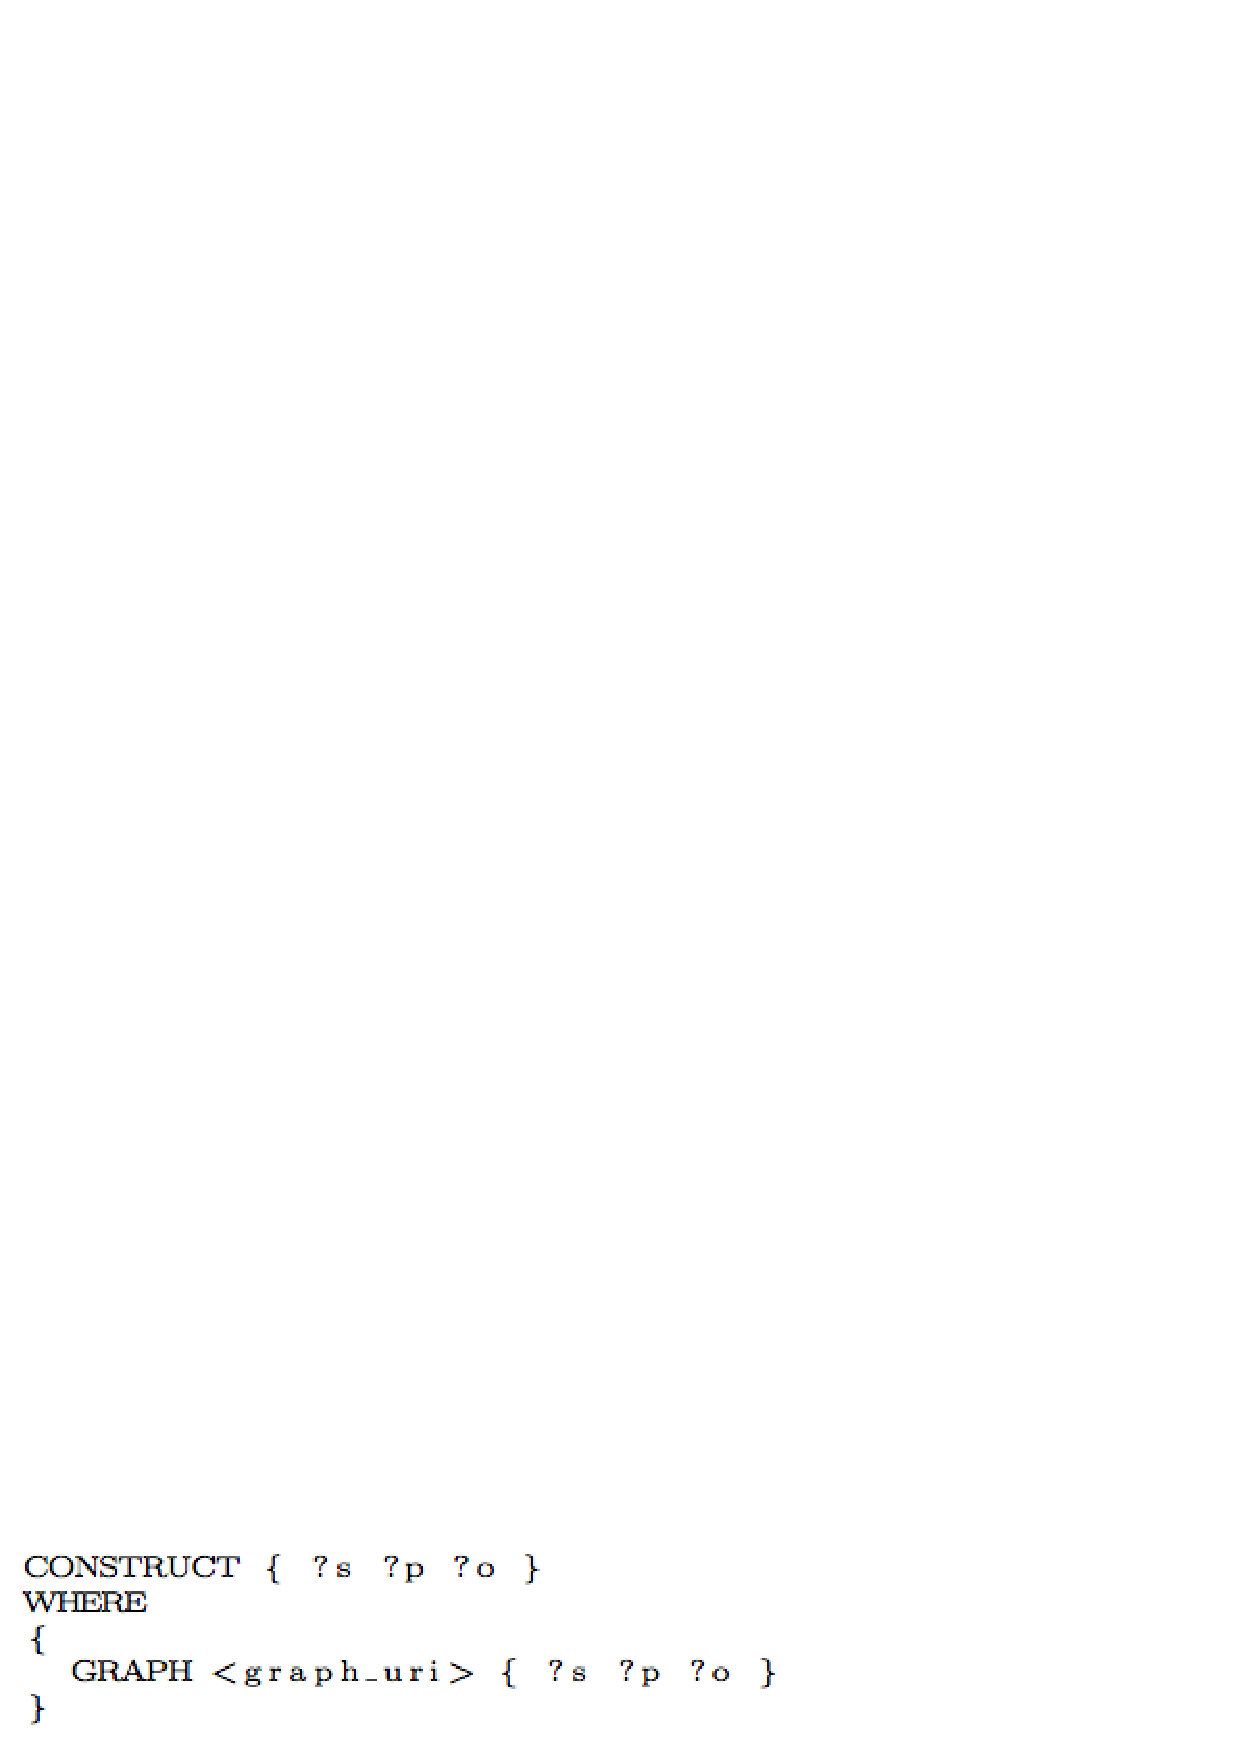
\includegraphics[width=0.8\textwidth]{tabla6}
\label{tabla6}
\end{table}


La sem\'antica de esta consulta \textit{SPARQL} coincide con la sem\'antica descrita en la propuesta de est\'andar \textit{Protocolo SPARQL HTTP Uniforme para la Gesti\'on de Grafos RDF} de la \textit{W3C}.\\
Adicionalmente, las peticiones \textit{GET} \textit{HTTP} pueden especificar dos par\'ametros \textit{\_pageSize} y textit{\_page} para modificar el n\'umero de tripletes en el grafo de destino que ser\'an recuperados por la consulta \textit{SPARQL} mediante el uso de las cl\'ausulas \textit{LIMIT} y \textit{OFFSET} del lenguaje \textit{SPARQL} al mismo tiempo que se ordena el conjunto de tripletes recuperados por sujeto, mediante el uso de la cla\'usula \textit{ORDER BY ?s}. Estos par\'ametros han sido propuestos en la propuesta \textit{LD-API} y permiten implementar paginaci\'on en el cliente \textit{HTTP} realizando la petici\'on.

\subsubsection{Peticiones \textit{POST}}

Las  peticiones \textit{HTTP} \textit{POST} para la creaci\'on de un nuevo recurso, son traducidas como peticiones \textit{INSERT DATA} del lenguaje \textit{SPARQL UPDATE} que insertar\'an los datos enviados en el cuerpo de la petici\'on \textit{HTTP} en un nuevo \textit{grafo con nombre} cuya \textit{URI} deber\'a generar el sistema, de acuerdo con el mecanismo de generaci\'on de identificadores elegido en la descripci\'on de la \textit{API}.\\
La sintaxis de la consulta \textit{SPARQL} UPDATE se muestra en la tabla \ref{tabla7}.\\

\begin{table}
\vspace{2.4in}
\caption{Consulta \textit{SPARQL} para una petici\'on \textit{HTTP} \textit{POST}.}
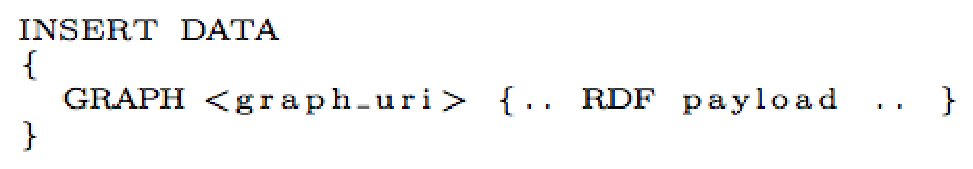
\includegraphics[width=0.8\textwidth]{tabla7}
\label{tabla7}
\end{table}

Una consideraci\'on importante es la distinci\'on que se debe hacer entre el \textit{URI} generado para identificar el \textit{grafo con nombre} que se almacenar\'a en el repositorio de grafos \textit{RDF} y el \textit{URI} que identifica el recurso \textit{RDF} en los tripletes almacenados ene el \textit{grafo con nombre} de acuerdo con la pr\'actica est\'andar a la que ha llegado la comunidad de Datos Enlazados Abiertos durante la discusi\'on de la relaci\'on entre recursos de informaci\'on y no recursos de informaci\'on \cite{fielding2005httprange}.\\
La siguiente tabla \ref{named_graph_vs_resource_uri} muestra las diferencias entre ambas \textit{URIs}.\\

\begin{table}
\centering
\caption{\textit{Grafos con nombre} frente a recursos \textit{RDF}.}
\label{named_graph_vs_resource_uri}
\begin{center}
\begin{tabular}{|l|l|}\hline
\textbf{\textit{Grafo con nombre}} & \textbf{\textit{Recurso RDF}} \\\hline
Identificado por un \textit{URI}. & Identificado por un \textit{URI}. \\
Recurso de informaci\'on. & No recurso de informaci\'on.\\
Identifica el \textit{grafo con nombre}. & Aparece dentro del \textit{grafo con nombre}.\\
Desreferenciable usando \textit{HTTP} & No desreferenciable usando \textit{HTTP}\\\hline
\end{tabular}
\end{center}
\end{table}


Sin embargo, ambas \textit{URIs} est\'an relacionadas, debiendo ser posible para un cliente web que se encuentre con la \textit{URI} del recurso formando parte de un triplete \textit{RDF} en otro grafo, seguir un enlace que desencadene una petici\'on \textit{HTTP} sobre la \textit{URI} del \textit{grafo con nombre} que almacena los datos del recurso.\\
Adem\'as, seg\'un los principios arquitect\'onicos \textit{REST}, la responsabilidad de generar la \textit{URI} del recurso \textit{HTTP}, lo que en nuestro caso significa generar un \textit{URI} para el \textit{grafo con nombre} y para el recurso \textit{RDF} almacenado en dicho grafo, depende del proveedor de la \textit{API}, no del cliente, por lo que la \textit{URI} del recurso \textit{RDF} no puede venir dada en los tripletes \textit{RDF} enviados por el cliente en la petici\'on \textit{HTTP}.\\
Nuestra soluci\'on a nuestro problema viene dada por un mecanismo que permite al cliente especificar un patr\'on de tripletes \textit{RDF} que se transformar\'a en el grafo \textit{RDF} final que se almacenar\'a en el repositorio \textit{RDF}, una vez que el servicio ha generado \textit{URIs} para el \textit{grafo con nombre} y el recurso \textit{RDF} mediante el mecanismo especificado en la descripci\'on de la \textit{API}.\\
El proceso es el siguiente:\\
\begin{itemize}

\item El cliente env\'ia una petici\'on \textit{HTTP} \textit{POST} a la \textit{URI} base de la colecci\'on de recursos, incluyendo un grafo \textit{RDF} en el cuerpo de la petici\'on, donde la \textit{URI} del recurso \textit{RDF} descrito en el grafo ha sido sustituido por un identificador de nodo an\'onimo \textit{RDF}. Adicionalmente, un par\'ametro \textit{\_self} se enviar\'a en la \textit{URI} de la petici\'on con el identificador del grafo an\'onimo usado para designar al recurso \textit{RDF} en el cuerpo de la petici\'on.
\item Si el grafo \textit{RDF} enviado en el cuerpo de la petici\'on incluye alg\'un triplete cuyo sujeto no es un identificador de nodo \textit{RDF} an\'onimo, el servicio debe devolver una respuesta de error \textit{HTTP} \textit{403 forbidden}.
\item El servicio genera una nueva \textit{URI} \textit{graph\_uri} para identificar al \textit{grafo con nombre} de acuerdo con el mecanismo especificado en la descripci\'on de la \textit{API}.
\item El servicio reemplaza el nodo an\'onimo especificada por el cliente en el patr\'on de tripletes \textit{RDF} para identificar el recurso \textit{RDF} por el \textit{hash URI} \cite{fielding2005httprange} \textit{graph\_uri\#self}.
\item El \textit{grafo con nombre} resultante, identificado por el \textit{URI} \textit{graph\_uri}, incluyendo la descripci\'on del recurso \textit{RDF} identificado por el \textit{URI} \textit{graph\_uri\#self} es almacenado en el repositorio \textit{RDF} mediante la consulta \textit{SPARQL Update} especificada en la tabla \ref{tabla7}.
\item Si la craci\'on del \textit{grafo con nombre}  resulta exitosa, el servicio debe devolver una respuesta \textit{HTTP} \textit{201 created} al cliente con una cabecera \textit{HTTP} \textit{location} con la \textit{URI} del nuevo \textit{grafo con nombre} creado.

\end{itemize}

El uso de un \textit{hash URI} para identificar al recurso \textit{RDF}, que usa como base el \textit{URI} utilizado para identificar al recurso \textit{HTTP} y al \textit{grafo con nombre} asociado, permite que clientes web que encuentran el \textit{URI} del recurso web enlazado en otro grafo \textit{RDF}, descubran el contenido del recurso \textit{RDF} sin desreferenciarlo directamente. Los \textit{hash URIs} no pueden ser directamente desereferenciadas. Cualquier intento de hacer una petici\'on \textit{HTTP} \textit{GET} a un \textit{hash URI} ser\'a interpretada por el servicio web como una petici\'on a la \textit{URI} base del \textit{hash URI}, en nuestro caso la \textit{URI} del \textit{grafo con nombre}, inici\'andose de esta manera el proceso de negociaci\'on de contenido \textit{HTTP} que finalmente llevar\'a al cliente a obtener una serializaci\'on concreta de la informaci\'on \textit{RDF} del recurso asociada al \textit{grafo con nombre}.

\subsubsection{Peticiones \textit{PUT}}

Las peticiones \textit{HTTP} \textit{PUT} son interpretadas por el servicio como un intento de reemplazar el contenido del recurso asociado por un nuevo contenido, en nuestro caso, un nuevo grafo \textit{RDF} que se almacenar\'a en el mismo \textit{grafo con nombre} asociado al recurso \textit{HTTP}.\\
Esta sem\'antica queda recogida en la combinaci\'on de consultas \textit{SPARQL Update} \textit{DROP SILENT} y \textit{INSERT DATA} sobre el repositorio de grafos \textit{RDF} en las que se traduce la petici\'on \textit{HTTP}. La tabla \ref{tabla8} muestra la sintaxis de dicha consulta.\\

\begin{table}
\vspace{2.4in}
\caption{Consulta \textit{SPARQL} para una petici\'on \textit{HTTP} \textit{PUT}.}
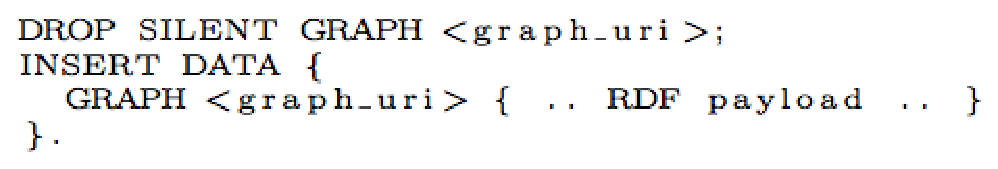
\includegraphics[width=0.8\textwidth]{tabla8}
\label{tabla8}
\end{table}

El cuerpo de la petici\'on \textit{PUT} debe contener s\'olo tripletes que usan como sujeto el identificador del recurso \textit{RDF} \textit{graph\_uri\#self} o identificadores de nodos an\'onimos \textit{RDF}. El servicio debe cancelar el procesamiento de la petici\'on y devolver un c\'odigo de error \textit{HTTP} \textit{403 forbidden} si esta condici\'on no se cumple.

\subsubsection{Peticiones \textit{DELETE}}

Por \'ultimo, las peticiones \textit{HTTP} \textit{DELETE} se traducen como peticiones \textit{DROP GRAPH} \textit{SPARQL}, que suponen la eliminaci\'on del \textit{grafo con nombre} y toda la informaci\'on asociada a dicho grafo. La tabla \ref{tabla9} muestra la sintaxis de la petici\'on.\\

\begin{table}
\vspace{2.4in}
\caption{Consulta \textit{SPARQL} para una petici\'on \textit{HTTP} \textit{DELETE}.}
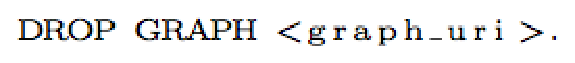
\includegraphics[width=0.8\textwidth]{tabla9}
\label{tabla9}
\end{table}


El procesamiento de la petici\'on \textit{HTTP} \textit{DELETE} supone la destrucci\'on del recurso \textit{HTTP} identificado por el \textit{URI} del \textit{grafo con nombre}. Cualquier petici\'on adicional a la \textit{URI} del recurso \textit{HTTP} debe ser resuelta por el servicio con una respuesta \textit{HTTP} \textit{404 not found}.

\subsection{Serializaci\'on de resultados}

Tras obtener una respuesta exitosa desde el repositorio de grafos \textit{RDF} mediante una consulta \textit{SPARQL} la implementaci\'on de la \textit{API} debe devolver la informaci\'on recuperada al cliente mediante la representaci\'on acordada entre cliente y servidor mediante el proceso de negociaci\'on de contenido especificado en el protocolo \textit{HTTP}.\\
Los tipos de contenido soportados por la especificaci\'on LD-API deben ser tambi\'en soportados como tipos v\'alidos por implementaciones de esta \textit{API}.\\
Un tipo de datos de especial inter\'es es el tipo de datos \textit{JSON}. \textit{JSON} es el formato de datos elegido por la mayor\'ia de \textit{APIs} de datos en uso hoy en d\'ia. Con el fin de asegurar que la \textit{API} va a resultar \'util para desarrolladores web no familiarizados con la pila de tecnolog\'ias sem\'anticas, que simplemente est\'an recuperando informaci\'on a trav\'es de la \textit{API}, es importante ofrecer una representaci\'on de los grafos \textit{RDF} como objetos \textit{JSON} que pueda ser utilizada con facilidad por parte de estos desarrolladores.\\
\textit{JSON-LD} \cite{jsonld} es una representaci\'on que cumple estos criterios, gracias especialmente a una caracter\'istica denominada coerci\'on de tipos que permite codificar los grafos \textit{RDF} como objetos \textit{JSON} sencillos, con una propiedad adicional en la que se incluye la traducci\'on entre propiedades simples del objeto \textit{JSON} y los \textit{URIs} de las propiedades \textit{RDF} y tipos de los literales. Desarrolladores consumiendo la \textit{API} y no interesados en estas caracter\'isticas sem\'anticas de los resultados obtenidos, pueden ignorar esta propiedad adicional y tratar los resultados obtenidos como objetos \textit{JSON} sencillos. \textit{JSON-LD} es la codificaci\'on elegida para la implementaci\'on de nuestro modelo de servicio para cualquier petici\'on \textit{HTTP} seleccionando \textit{JSON} como el tipo de representaci\'on elegido para el recurso que se quiere recuperar, o enviando informaci\'on codificada como \textit{JSON}.\\
Por \'ultimo, la \textit{API} tambi\'en soporta un par de par\'ametros adicionales en las peticiones que permiten modificar la representaci\'on del recurso solicitado fuera del mecanismo de negociaci\'on de contenido \textit{HTTP}:

\begin{itemize}

\item \textit{\_callback}: Par\'ametro que puede se pasado en la petici\'on y que forzar\'a al servicio a devolver una representaci\'on \textit{JSON-LD} del grafo \textit{RDF} asociado al recurso \textit{HTTP}, como el \'unico argumento de una invocaci\'on a una funci\'on \textit{JavaScript} cuyo nombre se pasa como valor del par\'ametro. Esta t\'ecnica, conocida como \textit{JSONP} \cite{jsonp}, permite a aplicaciones cliente \textit{JavaScript}, ejecut\'andose dentro de un navegador web sobrepasar la limitaci\'on impuesta por la pol\'itica de seguridad de dominio \'unico activa en todos los navegadores web.\\
\item \textit{\_format}: Especifica un tipo de representaci\'on, tomando precedencia sobre el valor especificado en la cabecera accept de la petici\'on \textit{HTTP}.

\end{itemize}

La presencia de estos par\'ametros adicionales que imponen una sem\'antica adicional fuera de lo especificado por el protocolo \textit{HTTP} se justifica por la existencia de clientes web con un control limitado sobre el uso del protocolo, como aplicaciones \textit{JavaScript} siendo ejecutadas dentro de un navegador web.

\section{Components Software}

En las dos secciones anteriores de este cap\'itulo hemos descrito un modelo formal para la descripci\'on de la computaci\'on basada en servicios \textit{REST} sem\'anticos y un modelo arquitect\'onico y de servicio que permite transformar el modelo formal en una arquitectura web en el que un conjunto de peticiones \textit{HTTP} recibidas desde una interfaz de red se transforman en peticiones \textit{SPARQL} sobre un repositorio de grafos \textit{RDF}.\\
Sin embargo, el modelo arquitect\'onico descrito no establece la naturaleza de los componentes software concretos que se deben emplear para implementar dicha arquitectura. En particular no se ha especifica ning\'un detalle sobre el repositorio de grafos \textit{RDF}, m\'as all\'a de que debe soportar consultas \textit{SPARQL 1.1 Update}. Tampoco se ha mencionado como un cliente web puede gestionar la informaci\'on \textit{RDF} recuperada por el servicio para llevar a cabo una computaci\'on como la descrita en  nuestro c\'alculo formal.\\
Siguiendo el esp\'iritu de la comunidad de Datos Enlazados Abiertos, en esta secci\'on examinaremos la implementaci\'on que hemos llevado a cabo de dos componentes software que ofrecen alternativas para implementar esos componentes de la arquitectura propuesta usando las tecnolog\'ias m\'as comunes hoy en d\'ia en el desarrollo web: los sistemas gestores de bases de datos relaciones como repositiorios de grafos \textit{RDF} y aplicaciones \textit{JavaScript} ejecut\'andose dentro de un navegador web como clientes.

\subsection{Ejecuci\'on de consultas \textit{SPARQL 1.1 UPDATE} sobre datos relacionales.}

Como vimos en el cap\'itulo dedicado al estado del arte en este documento, una de las contribuciones de la comunidad de Datos Enlazados Abiertos ha sido el desarrollo de la propuesta de recomendaci\'on \textit{W3C} \textit{R2RML} \cite{r2rml} para la traducci\'on de datos relaciones en tripletes \textit{RDF}.\\
\textit{R2RML} consiste en un vocabulario gen\'erico que puede usarse para transformar un esquema relacional en tripletes \textit{RDF}. Una descripci\'on formal simplificada de la sintaxis de \textit{R2RML} se muestra en la tabla \ref{tabla10} como una gram\'atica \textit{EBNF}.\\

\begin{table}
\vspace{2.4in}
\caption{Sintaxis \textit{EBNF} de \textit{R2RML}.}
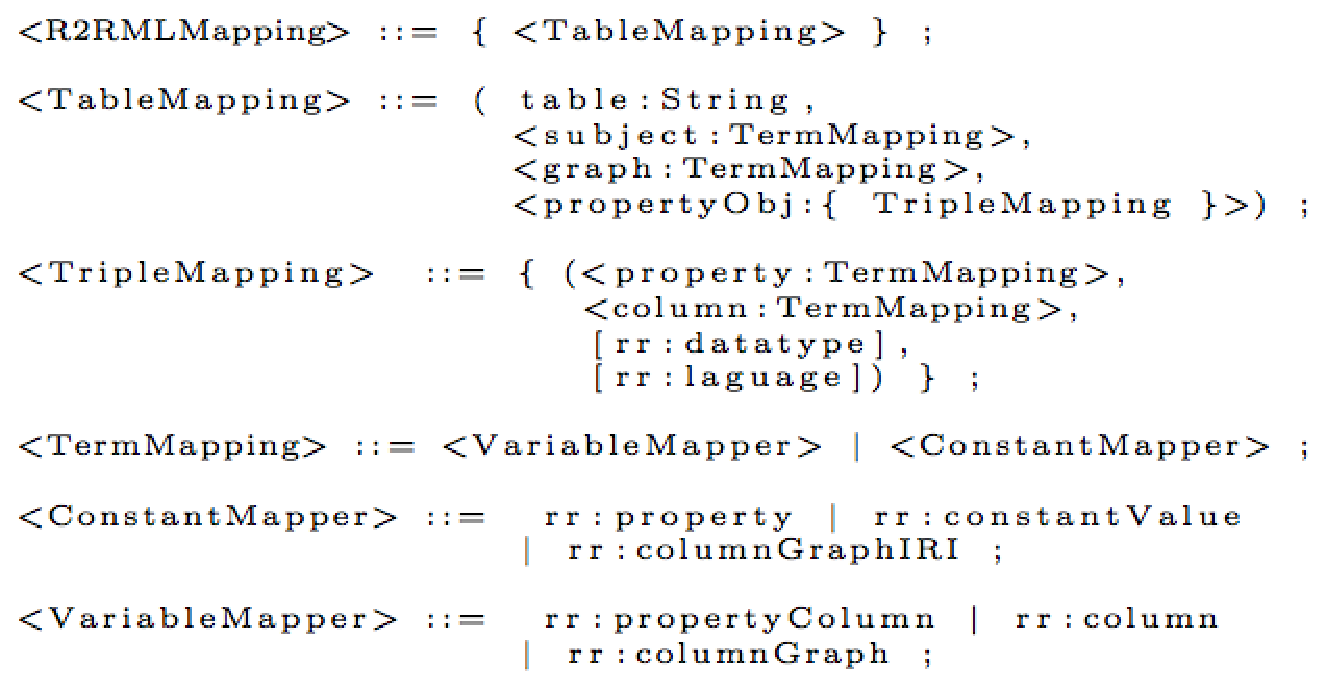
\includegraphics[width=0.8\textwidth]{tabla10}
\label{tabla10}
\end{table}


Este modelo formaliza \textit{R2RML} como una traducci\'on de una colecci\'on de \textit{TableMappings} por cada tabla del esquema relacional que se intenta transformar en tripletes \textit{RDF}. Cada \textit{TableMapping} describe como los datos almacenados en la tabla se deben transformar en \textit{quads} \textit{RDF}, tripletes aumentados consistentes en sujeto, predica, objeto y un \textit{grafo con nombre}. Los componentes de un \textit{quad} son generados usando un \textit{TermMapping} definido en el \textit{TableMapping}.\\
Cada \textit{TermMapping} puede ser constante o variable. Los \textit{TermMappings} constantes asignan un \textit{URI} o literal \textit{RDF} para el valor de ese componente en el quad \textit{RDF} que se va a generar. Por su parte los \textit{TermMappings} variables pueden hacer referencia a una columna en el esquema relacional de donde el valor para el componente del \textit{quad} ser\'a extra\'ido.
Por su parte, el est\'andar \textit{SPARQL 1.1 Update} describe un lenguaje com\'un para la recuperaci\'on y modificaci\'on de grafos \textit{RDF} con una sintaxis similar a la del lenguaje de consulta relacional \textit{SQL}. La principal unidad usada para construir consultas \textit{SPARQL} son los \textit{QuadPatterns} que pueden ser aplicados sobre los tripletes almacenados en un grafo \textit{RDF}. La tabla \ref{tabla11} formaliza la noci\'on de un \textit{QuadPattern} con sus posible componentes, variables y constantes.\\

\begin{table}
\vspace{2.4in}
\caption{Sintaxis de los \textit{QuadPatterns}.}
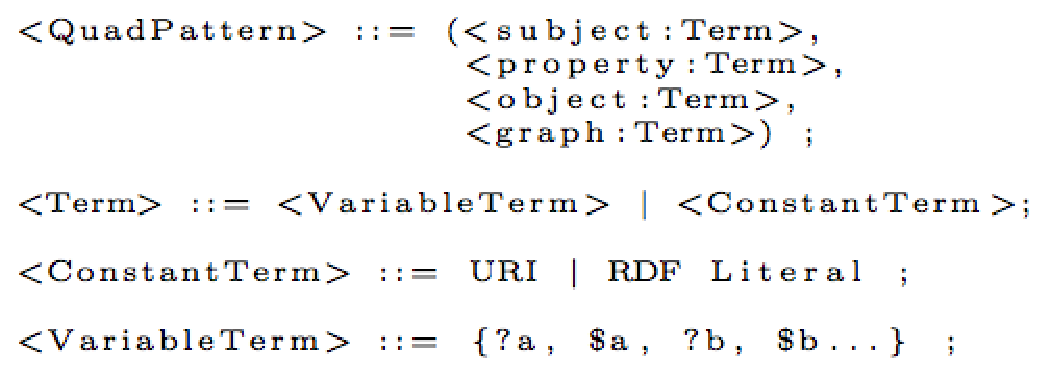
\includegraphics[width=0.8\textwidth]{tabla11}
\label{tabla11}
\end{table}


\textit{R2RML} describe una transformaci\'on desde el modelo relacional al modelo de datos de \textit{RDF}. Con el fin de usar un documento \textit{R2RML} para construir una transformaci\'on gen\'erica de consultas \textit{SPARQL 1.1 Update} sobre un grafo \textit{RDF} en consultas \textit{SQL} sobre un esquema relacional, es necesario describir una transformaci\'on inversa a la especificada por dicho documento \textit{R2RML}. La figura \ref{figura2} muestra el proceso propuesto para llevar a cabo esa transformaci\'on, as\'i como el papel que el documento \textit{R2RML} juega en dicho proceso.\\

\begin{figure}
\vspace{2.4in}
\caption{Diferentes transformaciones codificadas en un documento \textit{R2RML}}
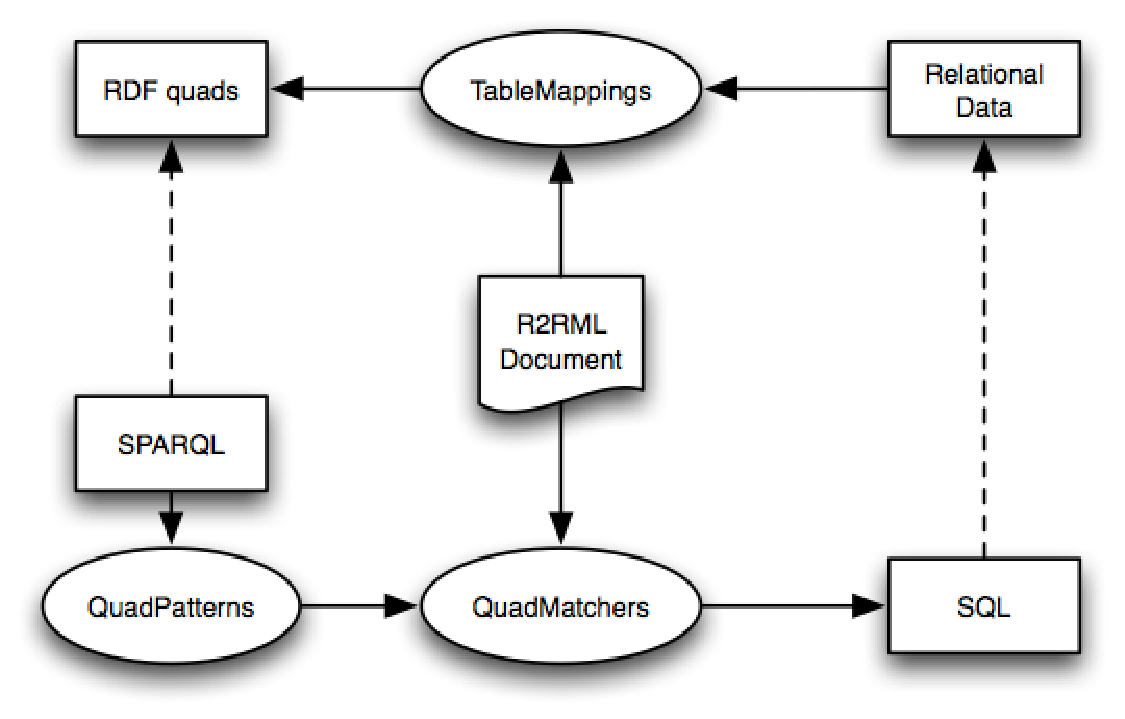
\includegraphics[width=0.5\textwidth]{figura2}
\label{figura2}
\end{figure}


El algoritmo descrito en la tabla \ref{alg1}, especifica en la funci\'on \textit{buildQuadMatchers} como llevar a cabo esa transformaci\'on inversa, generando un conjunto de \textit{QuadMatchers} para un conjunto de \textit{TripleMappers} de una descripci\'on \textit{R2RML} tomada como datos de entrada.\\

\begin{table}
\vspace{2.4in}
\caption{Algoritmo 1: Construcci\'on de \textit{QuadMatcher} para una tranformaci\'on \textit{R2RML}.}
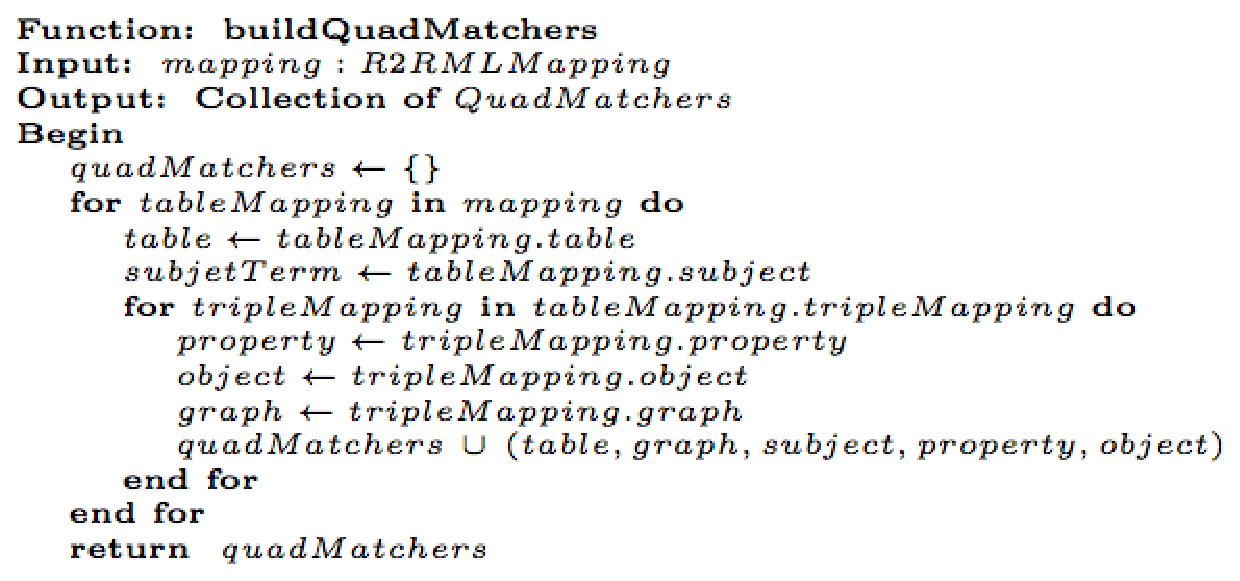
\includegraphics[width=0.8\textwidth]{algoritmo1}
\label{alg1}
\end{table}

El listado del algoritmo mostrado en la tabla \ref{alg2} describe a su vez un procedimiento para comprobar si un \textit{QuadMatcher} es compatible con un \textit{QuadPattern} en una consulta \textit{SPARQL}.\\

\begin{table}
\vspace{2.4in}
\caption{Algoritmo 2: Procedimiento para comprobar si un \textit{QuadPattern} y un \textit{QuadMatcher} son compatibles.}
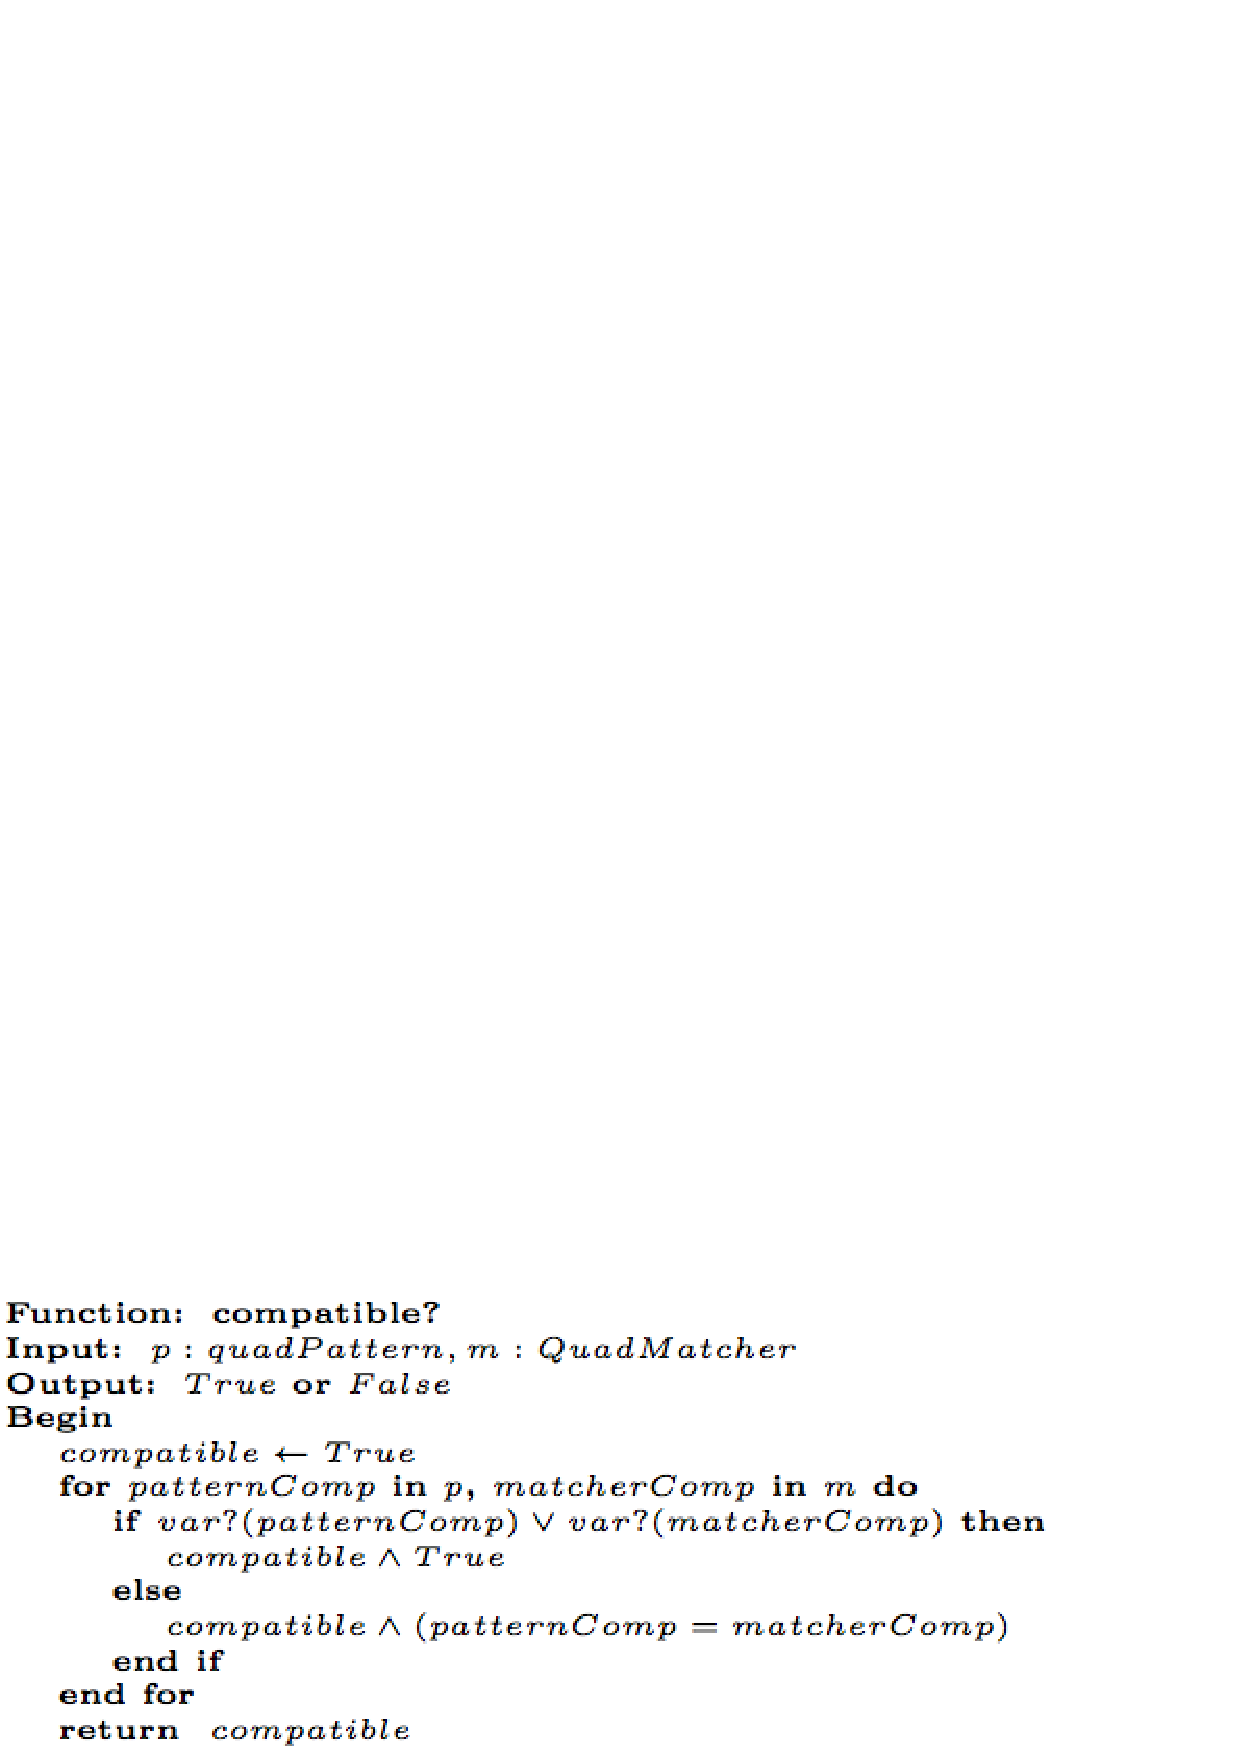
\includegraphics[width=0.8\textwidth]{algoritmo2}
\label{alg2}
\end{table}

En las siguientes secciones describiremos algoritmos que permiten usar la compatibilidad entre \textit{QuadMatchers} y \textit{QuadPatterns} para ejecutar consultas \textit{SPARQL} \textit{SELECT}, \textit{INSERT DATA} y \textit{DELETE} sobre datos relacionales con una transformaci\'on \textit{R2RML} asociada. Estas operaciones son suficientes para implementar las consultas sobre el repositorio de grafos \textit{RDF} descritas en la secci\'on anterior de este cap\'itulo como transformaciones de las operaciones \textit{HTTP} sobre recursos \textit{REST} sem\'anticos en el modelo arquitect\'onico de servicios propuesto. Las consultas \textit{DROP GRAPH} usadas en dicho modelo pueden ser transformadas en operaciones \textit{DELETE} equivalentes donde todos los tripletes del grafo son eliminados.

\subsubsection{Consultas \textit{SPARQL} \textit{SELECT}}

La transformaci\'on de consultas \textit{SPARQL} SELECT que proponemos se basa en el trabajo de \cite{chebotko2009semantics}, pero modificado para utilizar una transformaci\'on \textit{R2RML} como base, donde algunas de las restricciones que impone no son v\'alidas, como por ejemplo, el hecho de que la tabla de donde se extraen los componentes de un quad \textit{RDF} debe ser \'unica.\\
En el algoritmo de la tabla \ref{alg3} se muestra un procedimiento para transformar una consulta \textit{SPARQL SELECT} transformada en un conjunto de \textit{QuadPatterns} en una consulta \textit{SQL SELECT} mediante la b\'usqueda de los \textit{QuadMatchers} compatibles con los \textit{QuadPatterns} que luego son unidos mediante una cl\'ausula \textit{UNION} de \textit{SQL}.

\begin{table}
\vspace{2.4in}
\caption{Algoritmo 3: Composici\'on de una consulta \textit{SELECT} para un \textit{QuadPattern} y un conjunto de \textit{QuadMatchers}.}
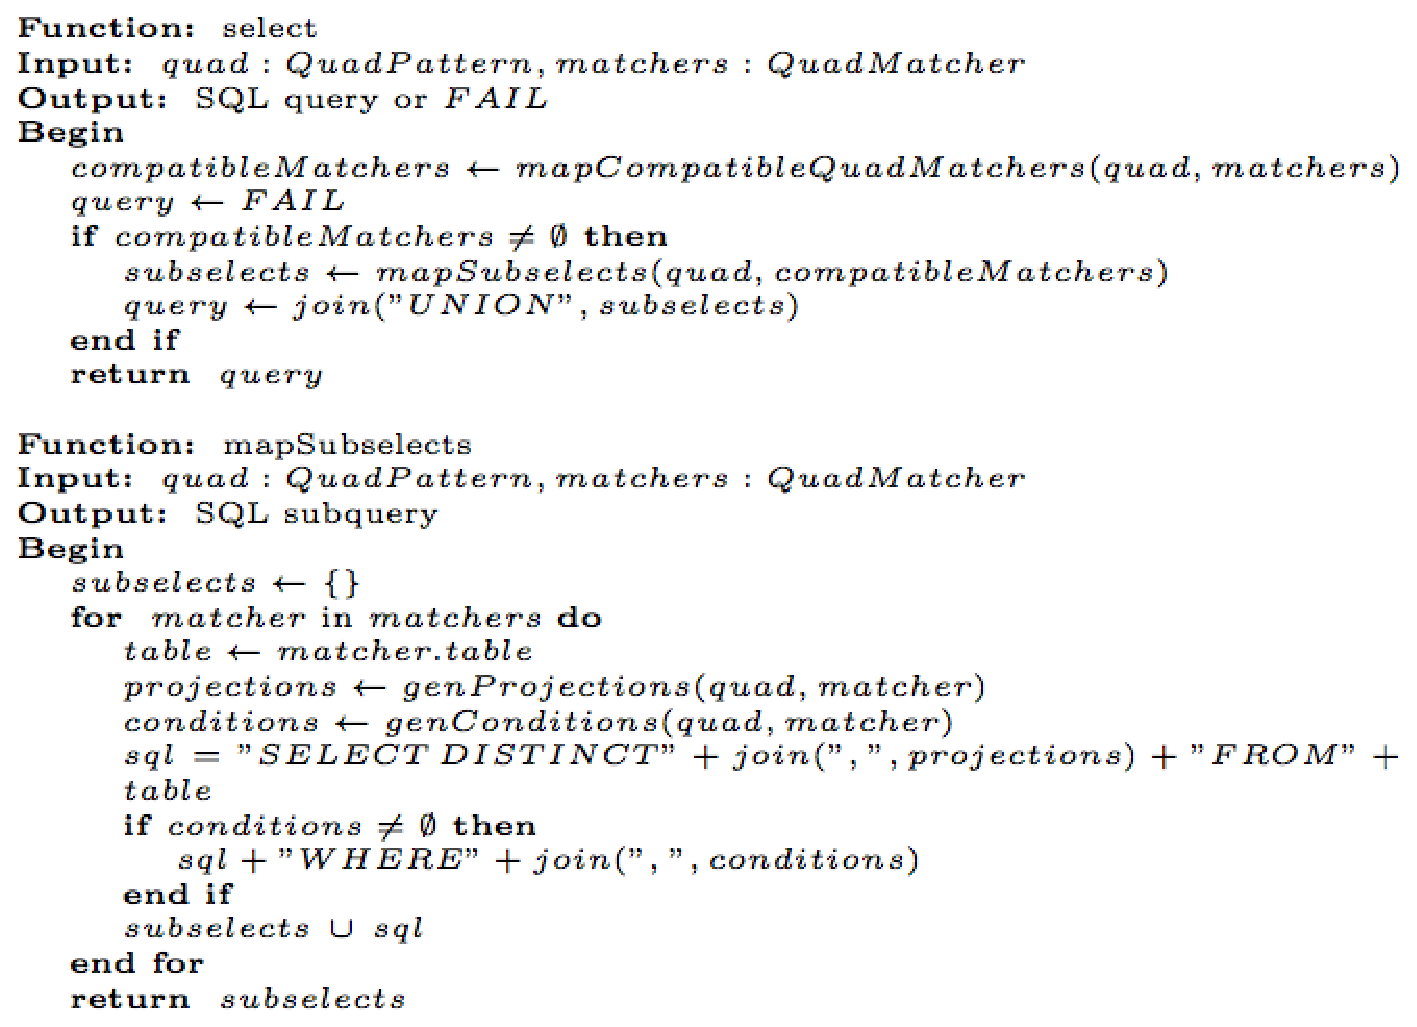
\includegraphics[width=0.8\textwidth]{algoritmo3}
\label{alg3}
\end{table}


\subsubsection{Consultas \textit{SPARQL} \textit{INSERT DATA}}

El la tabla \ref{alg4} contiene un algoritmo, que  muestra un procedimiento para la inserci\'on de un \textit{QuadPattern} con todos sus t\'erminos constantes en un esquema relacional con una transformaci\'on \textit{R2RML} asociada.\\

\begin{table}
\vspace{2.4in}
\caption{Algoritmo 4: Inserci\'on de un \textit{QuadPattern} para un conjunto de \textit{QuadMatchers}.}
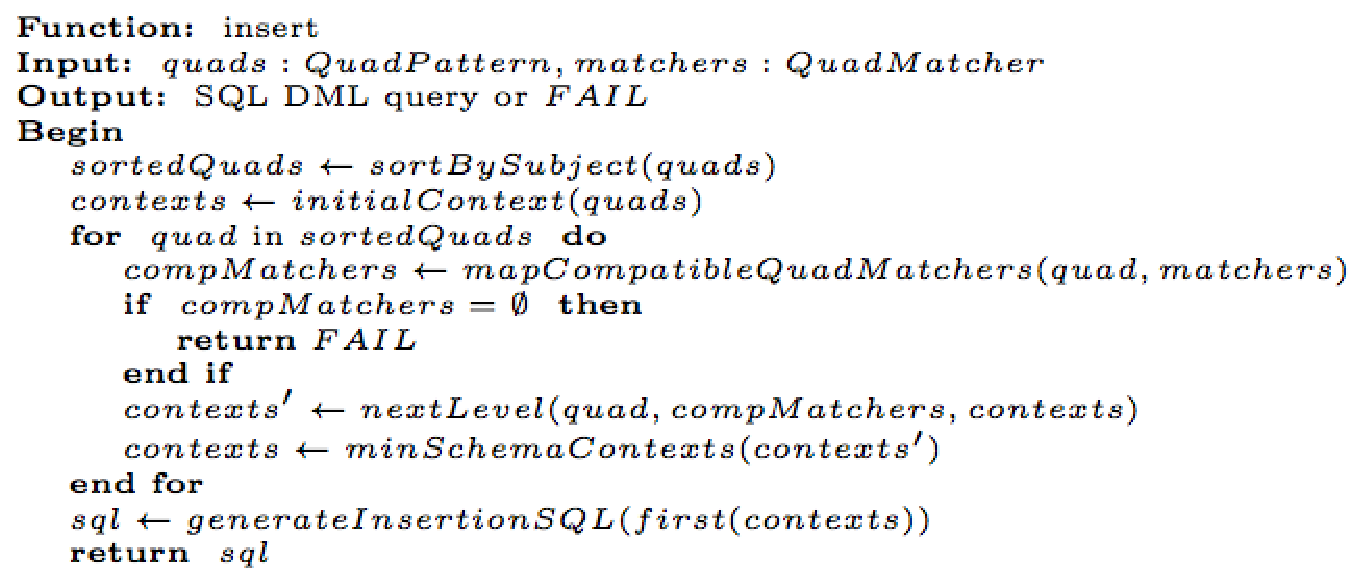
\includegraphics[width=0.8\textwidth]{algoritmo4}
\label{alg4}
\end{table}


El principal problema que se debe solucionar para llevar a cabo la inserci\'on es que es posible encontrar m\'as de un \'unico \textit{QuadMatcher} compatible con el componente del QuadPattern donde llevar a cabo la inserci\'on.\\
Como muestra la figura \ref{figura3}, el algoritmo propuesto funciona construyendo un \'arbol con las posibles opciones de inserci\'on encontradas y despu\'es selecciona aquella potencial inserci\'on que minimiza una m\'etrica de coste seg\'un descrita en el algoritmo de la tabla \ref{alg5}.

\begin{figure}
\vspace{2.4in}
\caption{Inserci\'on de dos \textit{quads}}
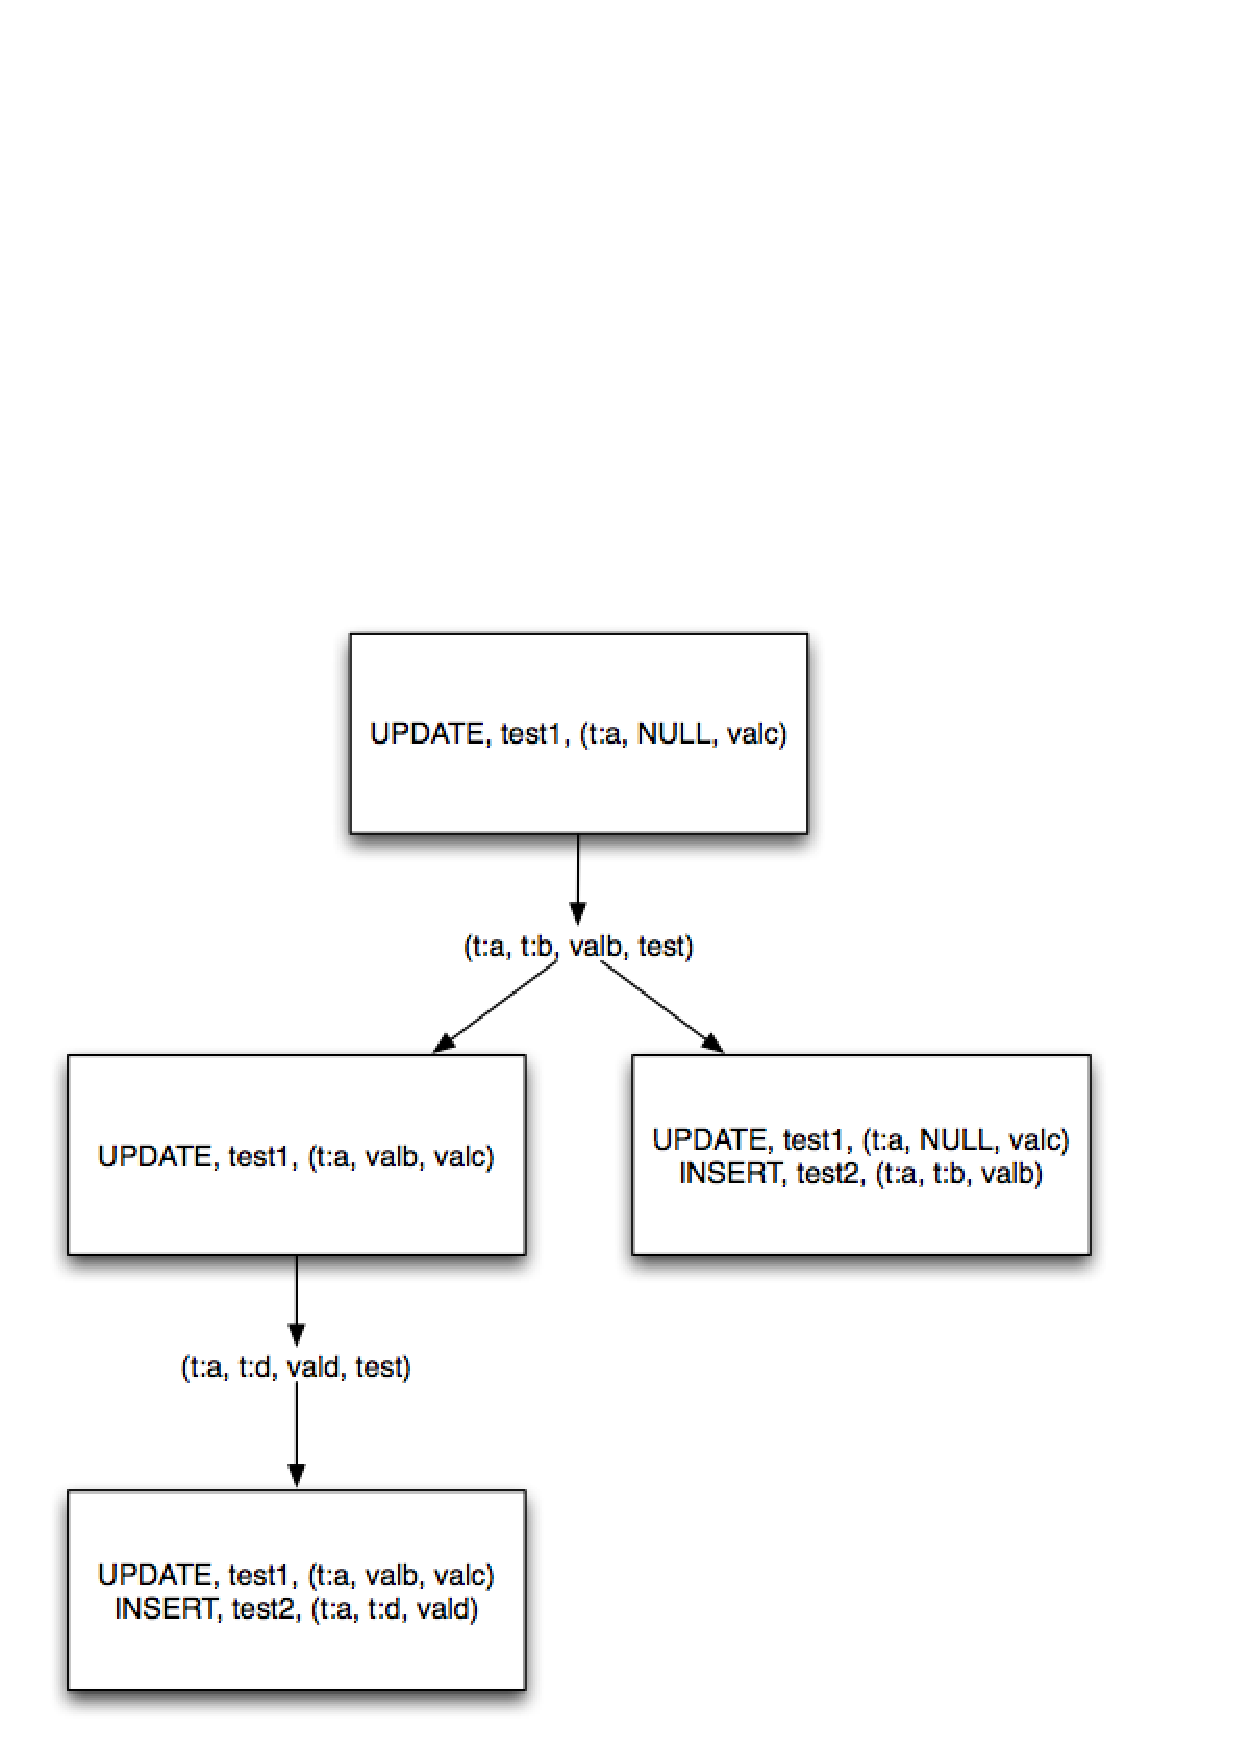
\includegraphics[width=0.5\textwidth]{figura3}
\label{figura3}
\end{figure}

\begin{table}
\vspace{2.4in}
\caption{Algoritmo 5: M\'etrica de coste.}
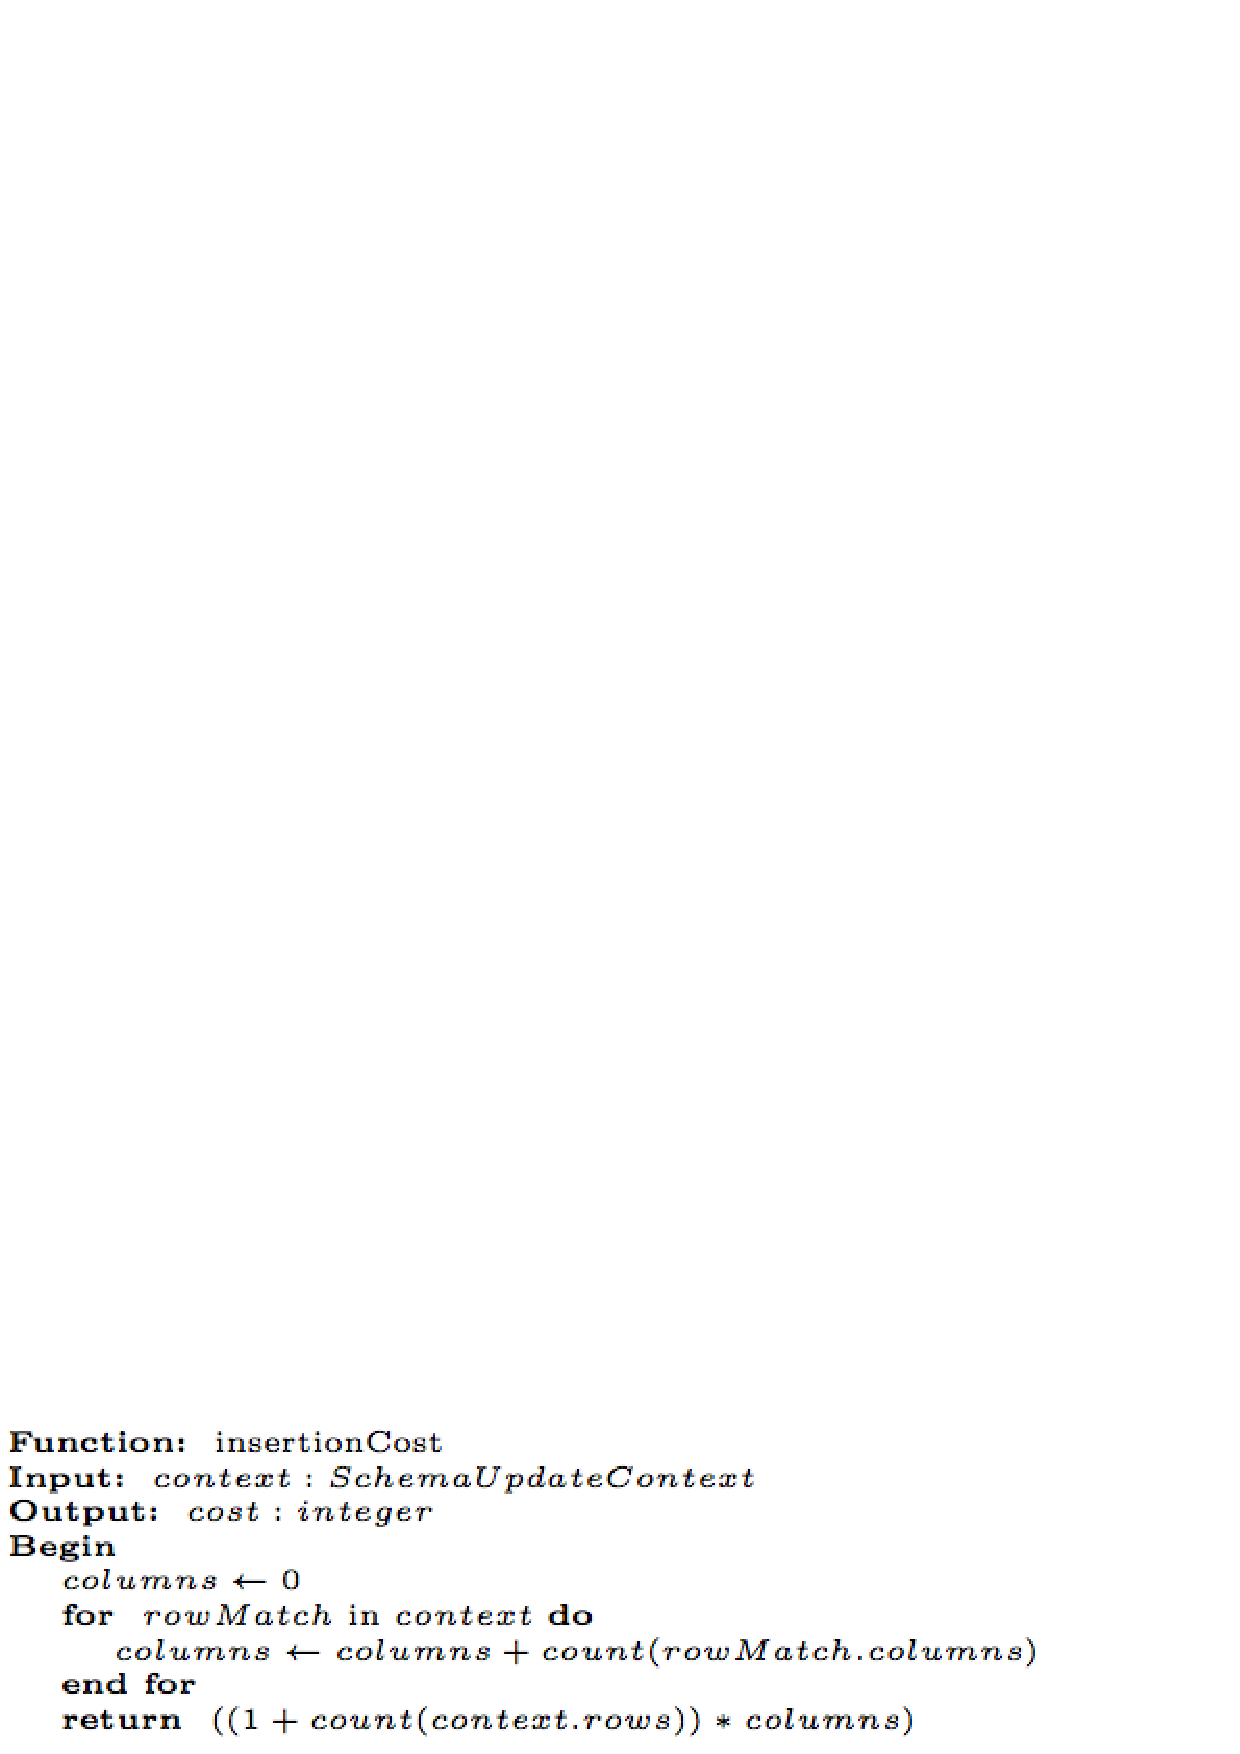
\includegraphics[width=0.8\textwidth]{algoritmo5}
\label{alg5}
\end{table}


\subsubsection{Consultas \textit{SPARQL} \textit{DELETE WHERE}}

Para traducir consultas \textit{DELETE} \textit{SPARQL} en consultas \textit{SQL} equivalentes dada una transformaci\'on \textit{R2RML} de un esquema relacional, el primer paso consiste en transformar la cl\'ausula \textit{WHERE} de la consulta \textit{SPARQL} en una consulta \textit{SELECT} \textit{SQL} y una vez ejecutada usando el algoritmo previamente descrito, usar los resultados obtenidos para aplicarlos sobre el patr\'on de la cl\'ausula \textit{SELECT} para obtener el conjunto final de quads que deben ser eliminados del grafo \textit{RDF}.\\
El algoritmo de la tabla \ref{alg6} describe un procedimiento para eliminar los quads almacenados en un esquema relacional con una transformaci\'on \textit{R2RML} asociada. El algoritmo actualiza las columnas de las tablas asociadas por la transformaci\'on \textit{R2RML} a las propiedades \textit{RDF} y objetos con valores nulos, en vez de eliminar todo el quad, ya que la columna sujeto puede ser compartida por otros tripletes almacenados en la misma fila.\\

\begin{table}
\vspace{2.4in}
\caption{Algoritmo 6: Composici\'on de una consulta para eliminar un \textit{QuadPattern} para un conjunto de \textit{QuadMatchers}.}
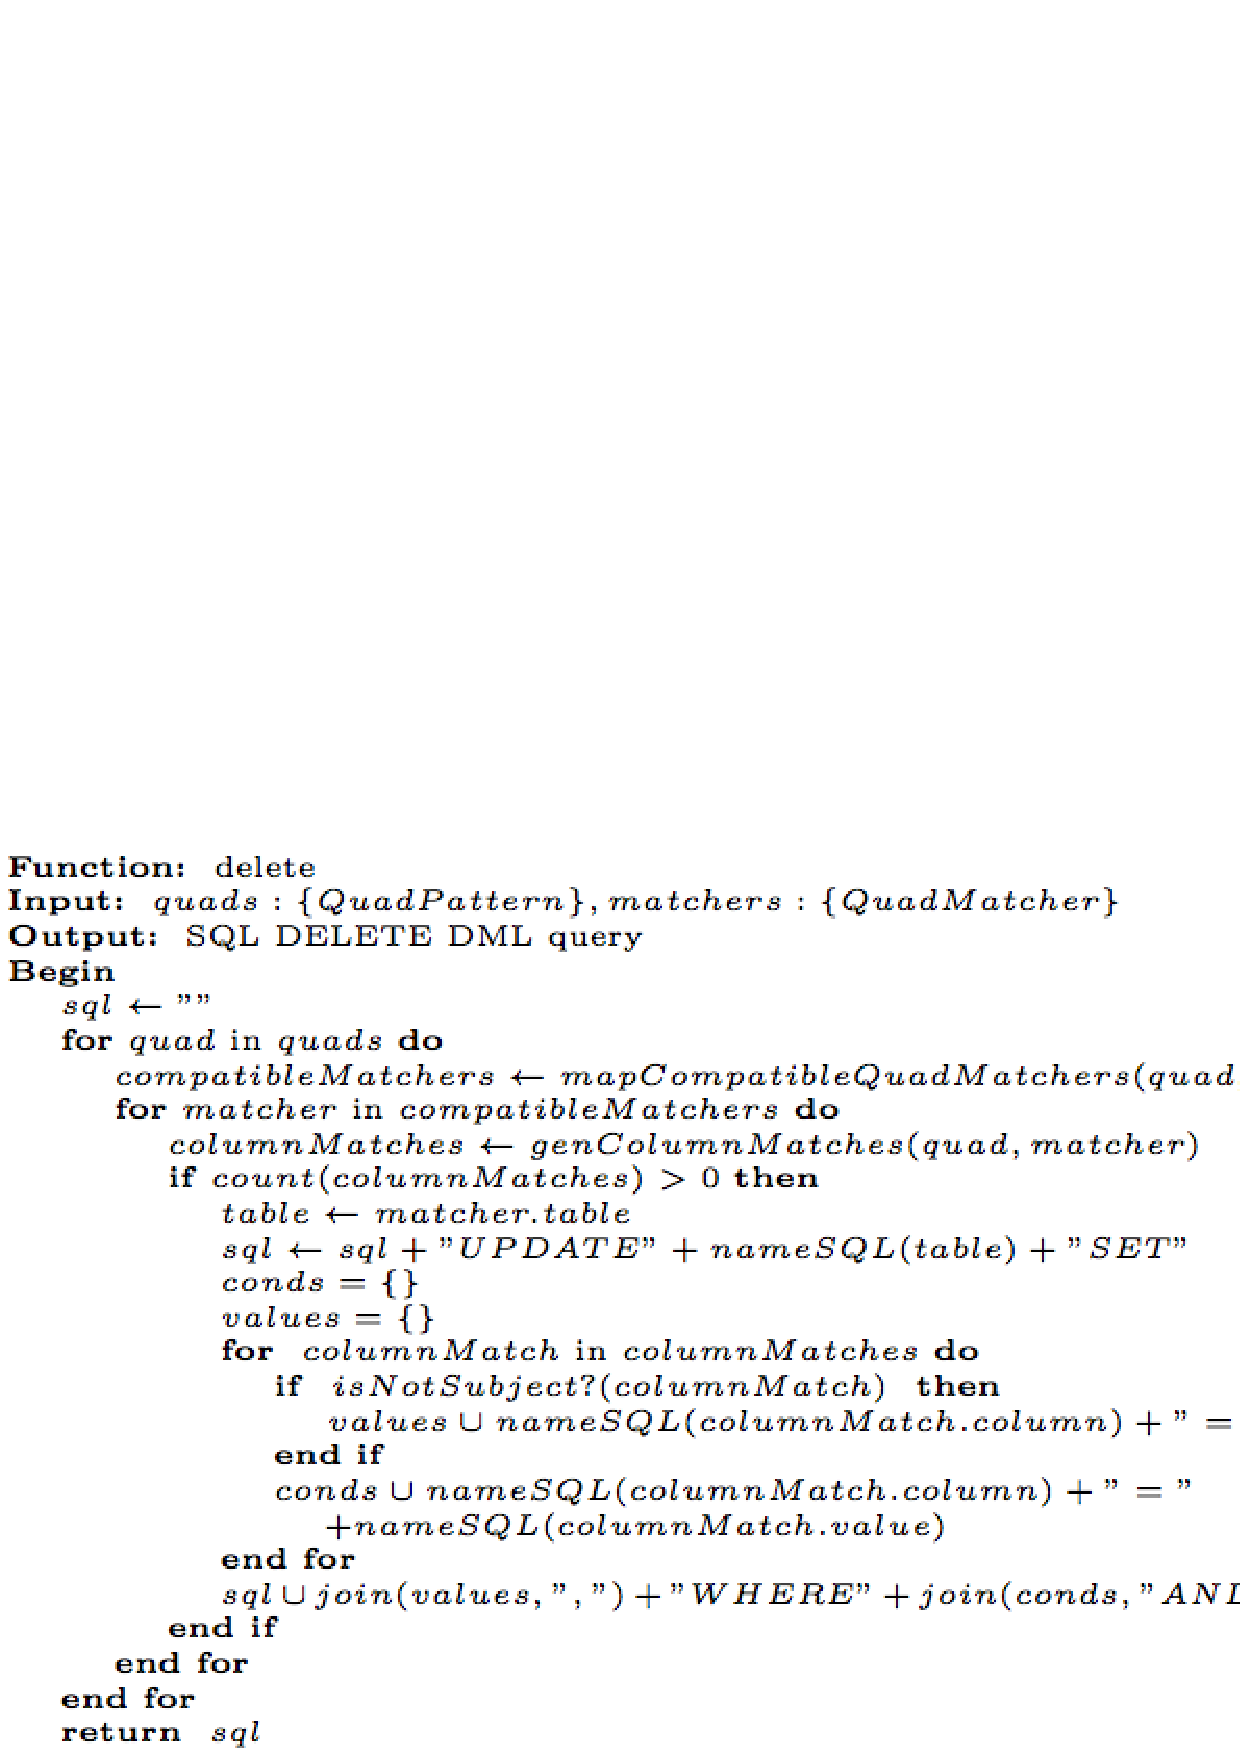
\includegraphics[width=0.8\textwidth]{algoritmo6}
\label{alg6}
\end{table}


Tras eliminar todos los quads, la funci\'on removeEmptyRows elimina todas aquellas filas en las tablas de la transformaci\'on \textit{R2RML} donde todos los valores para las columnas propieda y objeto tienen valores nulos.

\subsection{Un repositorio \textit{RDF} con soporte \textit{SPARQL 1.1 Update} para aplicaciones \textit{JavaScript}}

En secciones anteriores de este cap\'itulo hemos expuesto como, desde el punto de vista formal, una computaci\'on basada en recursos \textit{REST} sem\'anticos involucra tanto a procesos servicio, que exponen datos sem\'anticos a trav\'es de canales identificados con \textit{URIs} como a procesos cliente, que aunque no pueden ser accedidos directamente a trav\'es de \textit{URIs}, son capaces de consumir los datos sem\'anticos expuestos por los servicios y hacer avanzar la computaci\'on bas\'andose en los datos recuperados.\\
En la descripci\'on de la arquitectura que puede usarse para implementar el modelo te\'orico propuesto hemos hecho hincapi\'e en la parte servidor de la computaci\'on, sin entrar en los requisitos arquitecturales necesarios para implementar un proceso cliente capaz de consumir y tomar decisiones basadas en la informaci\'on sem\'antica recuperada.\\
En principio, los \'unicos requisitos necesarios para implementar un proceso cliente vienen dadas por los siguientes elementos b\'asicos:

\begin{itemize}
\item Soporte para el lado cliente del protocolo \textit{HTTP}.
\item Un mecanismo para almacenar grafos \textit{RDF} y ejecutar consultas \textit{SPARQL} sobre ellos.
\item Capacidad para reaccionar ante modificaciones en el grafo \textit{RDF} recuperado.
\end{itemize}

El soporte para el almacenamiento de grafos \textit{RDF} puede venir dado por el uso de un repositorio de grafos \textit{RDF} o un mecanismo que transforme un sistema gestor de bases de datos relacional en un repositorio \textit{RDF} con soporte para el lenguaje de consultas \textit{SPARQL}, como el que hemos expuesto anteriormente. Sin embargo, ning\'un tipo de repositorio \textit{RDF} de uso com\'un est\'a disponible para el que quiz\'as sea el m\'as com\'un de los entornos posibles para la ejecuci\'on de un proceso cliente en una computaci\'on basada en recursos \textit{REST} sem\'anticos: el navegador web.\\
En esta secci\'on describiremos nuestra implementaci\'on de un repositorio \textit{RDF} con soporte para el lenguaje de consultas \textit{SPARQL 1.1 Update} as\'i como para notificaciones as\'incronas asociadas a modificaciones en el grafo \textit{RDF} almacenado, que puede usarse como un componente de aplicaciones \textit{JavaScript} que son ejecutadas dentro del navegador web en general y en particular para aplicaciones clientes consumiendo la \textit{API} descrita en la secci\'on dedicada a la descripci\'on de una arquitectura de servicios web expuesta en este documento.\\
El repositorio est\'a contenido en una biblioteca \textit{JavaScript} que puede usarse como la base de la capa de datos en aplicaciones \textit{JavaScript} complejas ejecut\'andose en el navegador. La biblioteca soporta no solo el almacenamiento de grafos \textit{RDF} y la consulta de estos datos usando el lenguaje \textit{SPARQL 1.1 Update}, tambi\'en incluye funcionalidades para la deserializaci\'on de datos \textit{RDF} codificados usando formatos \textit{JSON}-LD, \textit{Turtle} y \textit{N3}.\\
La biblioteca se ha dise\~nado para tomar ventaja de las caracter\'isticas modernas que incluyen las \'ultimas versiones de los navegadores web, si se encuentran disponibles, como la ejecuci\'on multi-hilo mediante el soporte para \textit{WebWorkers} \cite{hicksonweb} y el almacenamiento de datos persistentes usando la funcionalidad de Web Storage \cite{webstorage}.\\
Otra interesante capacidad de la biblioteca consiste en la posibilidad de registrar funciones asociadas a eventos sobre el grafo, que ser\'an invocadas por el repositorio cuando una modificaci\'on en el grafo \textit{RDF} satisfaga las condiciones asociadas al evento.\\
Por \'ultimo, la implementaci\'on \textit{JavaScript} del repositorio permite su ejecuci\'on no s\'olo dentro del navegador web, sino tambi\'en en el lado servidor mediante una plataforma para la ejecuci\'on de aplicaciones \textit{JavaScript} conocida como \textit{Node.JS} que ha ganado una gran popularidad recientemente entre los desarrolladores de aplicaciones web. La figura \ref{figura4} muestra los principales componentes de la biblioteca que implementa el repositorio \textit{RDF}.

\begin{figure}
\vspace{2.4in}
\caption{Principales componentes del repositorio \textit{RDF}.}
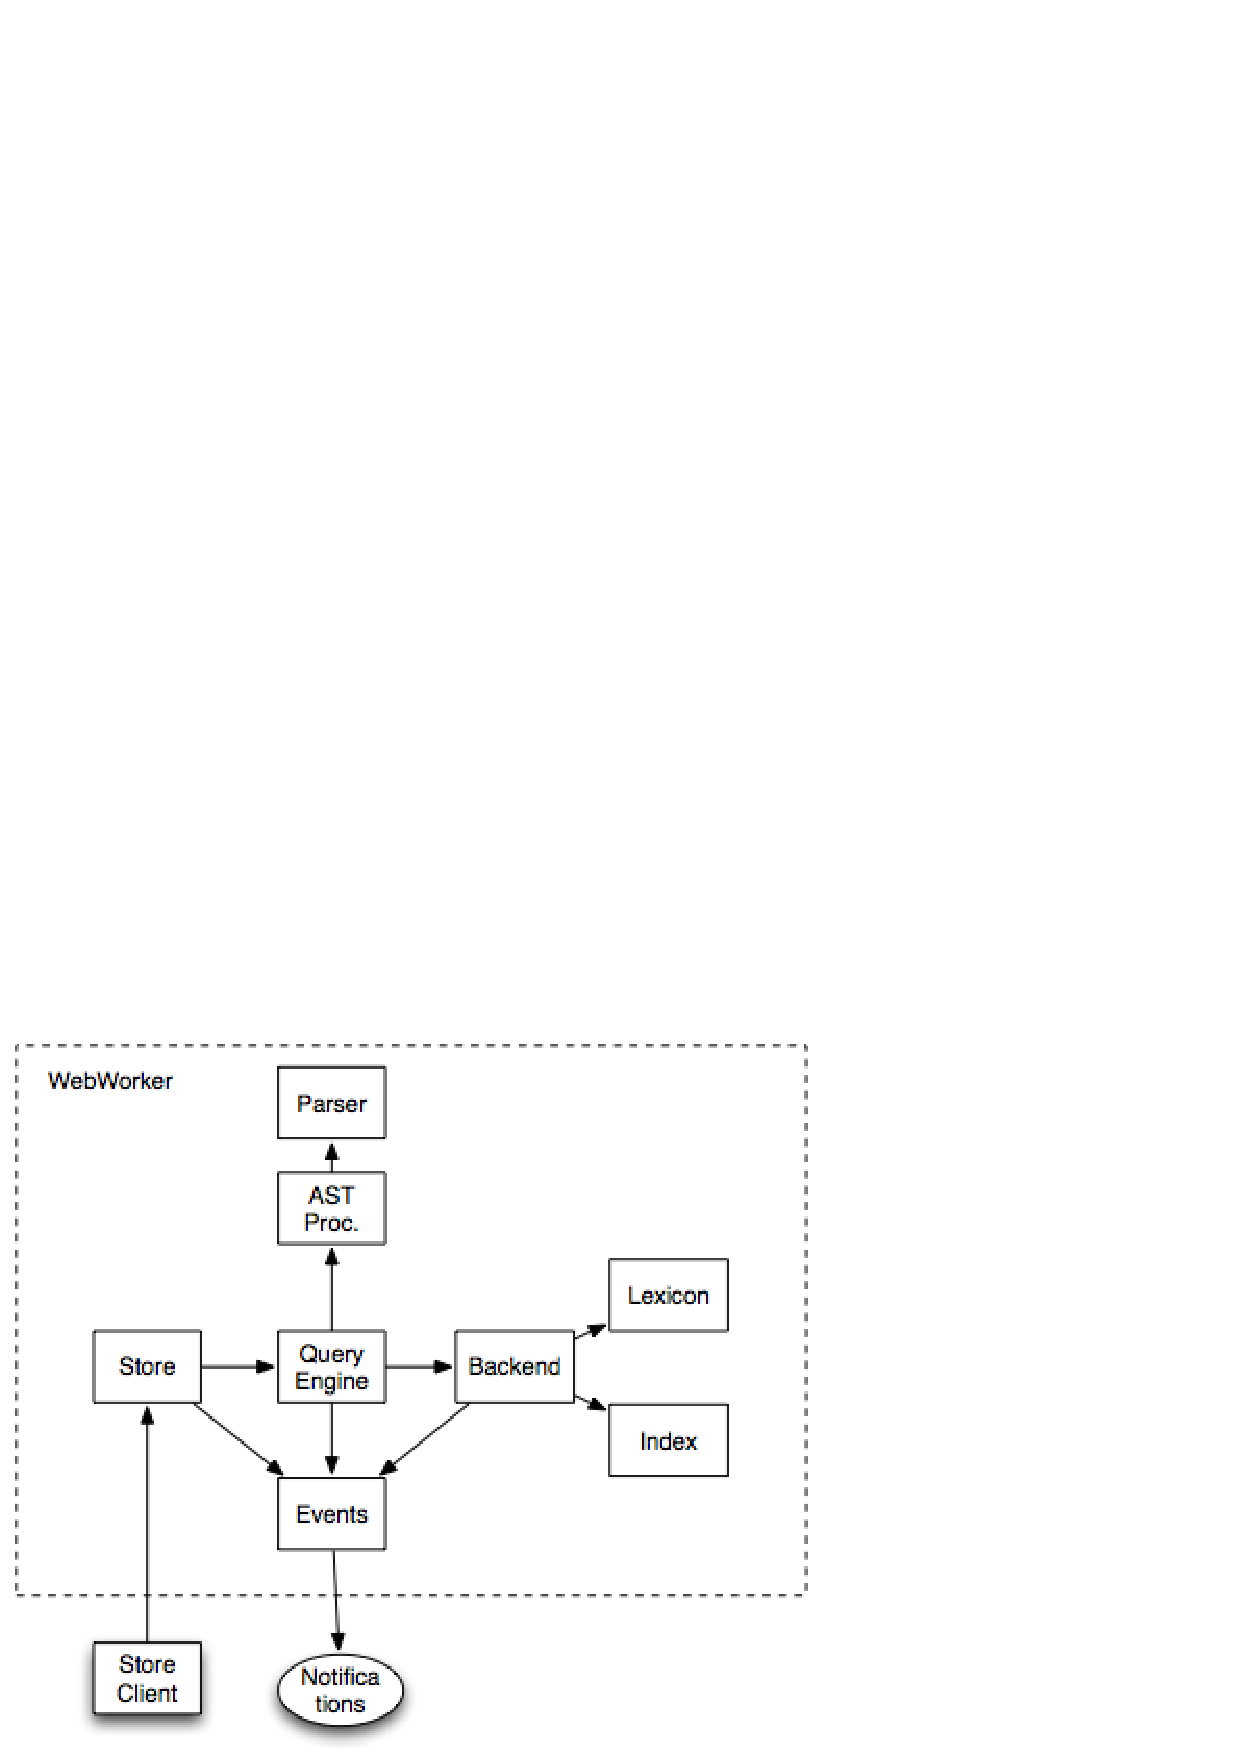
\includegraphics[width=0.5\textwidth]{figura4}
\label{figura4}
\end{figure}


\subsubsection{Almacenamiento persistente y no persistente}

El almacenamiento de datos en memoria no persistente de la biblioteca se basa en un modelo conceptual en el que todo los quads \textit{RDF} se almacenan en una \'unica tabla y son indexados usando un conjunto de estructuras de datos \textit{b-tree} que aumentan la eficiencia de las consultas de recuperaci\'on de datos.\\
Estos \'indices est\'an formados por el m\'inimo n\'umero de \'indices necesarios para cubrir los diferentes patrones presentes en las consultas \textit{SPARQL} formadas por patrones b\'asicos de grafo (\textit{BGP}) \cite{yars}.\\
En el almacenamiento persistente, hemos hecho uso de la \textit{API} de Web Storage \cite{webstorage}. Esta \textit{API} define un objeto \textit{JavaScript} \textit{localStorage} que recubre un mapa persistente donde se pueden almacenar pares clave-valor como objetos \textit{String} \textit{JavaScript}. La capacidad de almacenamiento de este mapa es limitado, siendo 15 MB el l\'imite por defecto presente en la mayor\'ia de los navegadores web modernos. La tabla de datos y los \'indices son almacenados en esta capa de persistencia usando un mecanismo propio que permite la serializaci\'on eficiente de los componentes de los \textit{quads} \textit{RDF} como objetos \textit{JSON}. Al mismo tiempo, un componente de \textit{cach\'e} permite un acceso eficiente a los datos almacenados reduciendo el n\'umero de b\'usquedas necesarios en la capa de persistencia.

\subsubsection{Procesamiento de consultas \textit{SPARQL}}

La ejecuci\'on de una consulta \textit{SPARQL} sobre un grafo \textit{RDF} almacenado en el repositorio se realiza en dos pasos diferenciados por la biblioteca.\\
En primer lugar se lleva a cabo el an\'alisis del texto de la consulta \textit{SPARQL} que es transformado en un objeto \textit{JSON} complejo que representa el \'arbol de sintaxis abstracta para la consulta. Este paso se ha implementado usando una \textit{Parsing Grammar Expression} (\textit{PEG}) \cite{pegs} con capacidad para analizar l\'exicamente consultas \textit{SPARQ 1.1 Update} y documentos \textit{Turtle}.\\
A continuaci\'on, el \'arbol de sintaxis abstracta es transformado en un objeto \textit{JSON} diferente que contiene la representaci\'on de una expresi\'on en el \'algebra \textit{SPARQL} \textit{cyganiak2005relational} equivalente de acuerdo con la sem\'antica para \textit{SPARQL} estandarizada por la \textit{W3C}.\\
Esta expresi\'on algebraica sera el objeto de procesamiento por el motor de ejecuci\'on \textit{SPARQL} del repositorio, que realizar\'a las consultas adecuadas sobre la tabla l\'exica y los \'indices del repositorio para generar los resulados finales de la consulta y serializarlos en el formato deseado por el cliente.

\subsubsection{Ejecuci\'on multi-hilo}

Las aplicaciones \textit{JavaScript} ejecut\'andose en el navegador se encuentran limitadas a un \'unico hilo de ejecuci\'on. Un posible mecanismo para sobrellevar esta limitaci\'on se encuentra en la \textit{API} de \textit{WebWorkers} \cite{hicksonweb} presente en las \'ultimas versiones de la mayor\'ia de navegadores web. Esta \textit{API} hace posible ejecutar c\'odigo \textit{JavaScript} en un hilo de ejecuci\'on diferente con severas restricciones en cuanto a las capacidades del navegador que ese hilo puede utilizar. El hilo principal de la aplicaci\'on y estos hilos especiales y \textit{REST}ringidos se comunican mediante un protocolo de paso de mensajes.\\
La biblioteca que implementa el repositorio se beneficia del soporte para \textit{WebWorkers}, si est\'a disponible, para ejecutar consultas \textit{SPARQL} de una manera concurrente en un conjunto de hilos restringidos. Desde el punto de vista de la arquitectura de la biblioteca, la interfaz entre cliente y repositorio est\'a implementado en un componente que sirve de fachada al sistema. Si el soporte para \textit{WebWorkers} es detectado, un conjunto de hilos \textit{REST}ringidos es creado y las consultas son distribuidos entre ellos. Cuando el procesamiento de una consulta ha finalizado, el resultado es pasado al componente fachada que finalmente env\'ia los resultados al cliente. Si el soporte para \textit{WebWorkers} no est\'a presente, la l\'ogica presente en los hilos restringidos es cargada por el componente fachada en el hilo principal y se procede a ejecutar las consultas \textit{SPARQL} de una manera secuencial.\\
Como ya hemos comentado, los hilos creados a trav\'es de la \textit{API} \textit{WebWorkers} se encuentran muy limitados, no pudiendo, por ejemplo, realizar peticiones web o acceder a la \textit{API} \textit{WebStorage}. Cuando un hilo \textit{REST}ringido necesita llevar a cabo cualquiera de estas operaciones, un mensaje debe ser enviado al hilo principal para que la lleve a cabo y env\'ie el resultado al hilo \textit{REST}ringido de modo que pueda continuar con su ejecuci\'on.

\subsubsection{\textit{API} de eventos}

Las aplicaciones \textit{JavaScript} presentan un modelo de ejecuci\'on reactivo, donde el c\'odigo escrito de forma as\'incrona, es ejecutado como respuesta a eventos sucedidos en la aplicaci\'on.\\
Nuestra implementaci\'on de un repositorio \textit{RDF} para \textit{JavaScript} hace posible usar este modelo de ejecuci\'on as\'incrono, permitiendo que la aplicaci\'on registre funciones que ser\'an ejecutadas cuando un determinado evento suceda en el grafo \textit{RDF} almacenado en \'el.\\
Este modelo de ejecuci\'on tambi\'en se encuentra pr\'oximo al modelo te\'orico que hemos presentado donde diferentes procesos se comunican a trav\'es de un espacio de tripletes a trav\'es de operaciones de lectura y escritura sobre \'el.\\
El mecanismo de eventos funciona a dos niveles de abstracci\'on diferentes: al nivel de las consultas \textit{SPARQL} y al nivel de los nodos \textit{RDF}.\\
Desde el punto de vista puramente \textit{SPARQL}, el cliente puede subscribirse a una consulta \textit{SPARQL} que ser\'a evaluada continuamente por el repositorio. Cada vez que una modificaci\'on del grafo \textit{RDF} modifique los resultados de la consulta, la funci\'on subscrita a la consulta ser\'a invocada de nuevo con el nuevo resultado para la misma.\\
Al nivel de los nodos \textit{RDF}, un cliente puede subscribirse a un nodo \textit{RDF} particular, identificado por un \textit{URI}, siendo notificado con el nuevo estado del nodo cada vez que una modificaci\'on del grafo \textit{RDF} haga que los contenidos o la misma presencia del nodo en el grafo cambie.

\subsubsection{Evaluaci\'on de rendimiento}

Como parte final del proceso de desarrollo del repositorio, hemos realizado una evaluaci\'on de rendimiento de la biblioteca utilizando el modelo de evaluaci\'on \textit{LUBM} \cite{lubm} ajustado sus par\'ametros para usar un conjunto de datos peque\~no. La evaluaci\'on se ha realizado para diferentes navegadores web en un equipo port\'atil medio.\\
Los casos de prueba se han generado autom\'aticamente mediante el generado de datos incluido dentro de \textit{LUBM} y a continuaci\'on se han transformado en \textit{JSON-LD} antes de ser cargados en el navegador para su ejecuci\'on. La cantidad final de tripletes almacenados en un \'unico grafo en el repositorio ha sido de 100545 tripletes. La tabla \ref{tabla12} muestra los resultados obtenidos en milisegundos para las diferentes consultas \textit{LUBM}.\\

\begin{table}
\vspace{2.4in}
\caption{Pruebas de rendimiento \textit{LUBM} para el repositorio \textit{RDF}}
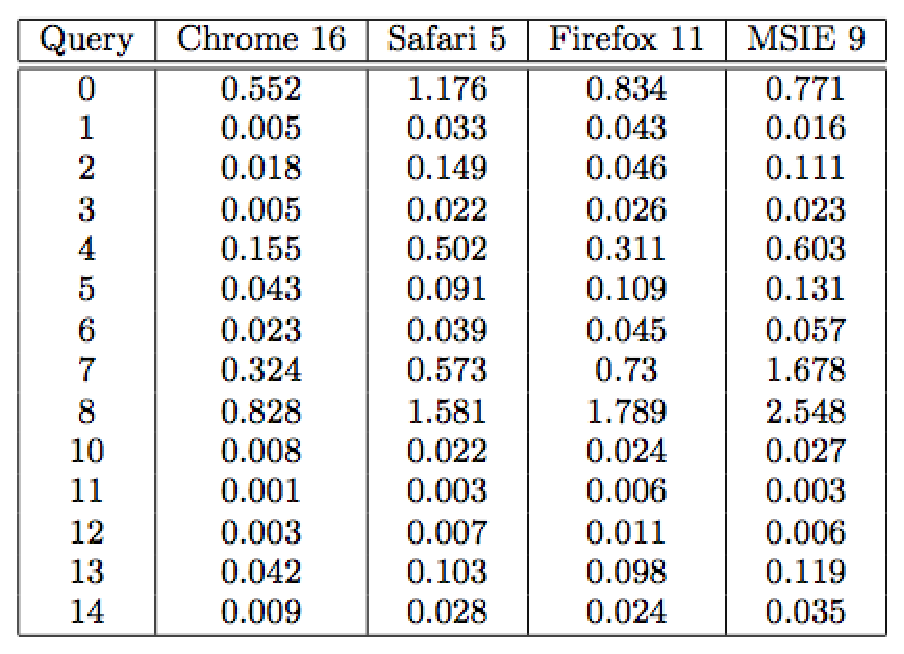
\includegraphics[width=0.8\textwidth]{tabla12}
\label{tabla12}
\end{table}

 Dado que el repositorio no soporta inferencia l\'ogica, algunas consultas en \textit{LUBM} han debido ser re-escritas para utilizar cl\'ausulas \textit{UNION} con el fin de cubrir todos los casos y obtener los resultados correctos esperados. Una consulta adicional que simplemente devuelve todos los tripletes ha sido tambi\'en a\~nadida. El texto de las consultas as\'i como el c\'odigo para ejecutar las consultas forma parte de la distribuci\'on de la biblioteca.

\section{Ejemplos de aplicaci\'on}

En las secciones anteriores de este documento hemos abordado el problema de la construcci\'on de \textit{APIs} de datos enlazados sem\'anticos desde la definici\'on de un modelo formal y un modelo arquitect\'onico hasta el dise\~no de componentes software que permitan implementar dicha arquitectura en una soluci\'on real.\\
En este apartado mostraremos ejemplos concretos de como estos elementos pueden ser usados para construir aplicaciones software que hacen uso de las ventajas que la existencia de una \textit{API} de datos enlazados sem\'anticos para ofrecer nuevas soluciones a dominios de aplicaci\'on reales, como la construcci\'on de aplicaciones web sociales o la implementaci\'on de sistemas para visualizaci\'on de la informaci\'on en el navegador.\\
En todos los casos haremos un breve repaso de los problemas que el actual estado de implementaci\'on de este tipo de aplicaciones presenta para despu\'es centrarnos en que ventajas aporta el uso de datos enlazados sem\'anticos y de la implementaci\'on de dicha soluci\'on en el marco tecnol\'ogico propuesto anteriormente en este documento.

\subsection{Un servidor personal de datos enlazados sem\'anticos para la Web Social}

La Web Social est\'a compuesta hoy en d\'ia por un n\'umero ingente de diferentes servicios donde los usuarios mantienen fragmentos de su grafo social. La interoperabilidad entre diferentes redes sociales es un importante problema sin resolver en el dise\~no de la Web Social vigente hoy en d\'ia. Desde el punto de vista del acceso a los datos, la mayor\'ia de las web sociales pueden considerarse silos de informaci\'on \cite{halpin2008beyond} donde la posibilidad de compartir datos a trav\'es aplicaciones se ve dificultada por mecanismos de autenticaci\'on, \textit{APIs}  y modelos de datos incompatibles.\\
La misma identidad de los usuarios tambi\'en se encuentra fragmentada entre aplicaciones. Diferentes mecanismos de autenticaci\'on y credenciales de usuario son usadas para identificar al usuario en diferentes redes sociales. Como resultado, funcionalidades como la importaci\'on del grafo social de contactos de una red social d\'onde ya se es miembro a un nuevo servicio es una tarea compleja que los usuarios deben completar antes de que puedan empezar a utilizar el nuevo servicio de una forma satisfactoria, convirti\'endose de esta manera en un importante barrera de entrada en la adopci\'on de nuevos servicios.\\
A pesar de los esfuerzos de estandarizaci\'on a los niveles de \textit{API}  e identidad, como OAuth \cite{hammer2010oauth} y OpenID \cite{openid}, la tendencia reciente consiste en concentrar la autenticaci\'on de los usuarios en un peque\~no conjunto de proveedores de identidad como \textit{Google}, \textit{Twitter} o \textit{Facebook}. Una consecuencia de esta tendencia es que no solo los datos sociales de los usuarios del servicio sino tambi\'en la misma identidad del usuario es retenida por un peque\~no conjunto de proveedores de servicios web, con el riesgo que esto supone de perdida de esa identidad si el servicio desaparece o la subordinaci\'on de los intereses del usuario a las pol\'iticas corporativas de dichas compa\~n\'ias.\\
En esta secci\'on describiremos como un servicio basado en una \textit{API} de datos enlazados sem\'anticos, basadas en est\'andares desarrollados por las comunidades Web Sem\'antica y Datos Enlazados Abiertos, en conjunci\'on con otras propuestas recientes aparecidas en el seno de dichas comunidades como \textit{WebID}, puede ser una alternativa viable para la construcci\'on de redes sociales descentralizadas donde los usuarios tengan un mayor control sobre su identidad en la web y grafo social.\\
En concreto, el sistema descrito a continuaci\'on es capaz de recoger datos sociales de diferentes servicios en los que el usuario est\'a registrado, transformando todos estos datos diversos en un \'unico grafos social usando un modelos de datos y una sem\'antica unificadas. El sistema asocia tambi\'en dicho grafo a un identidad \textit{WebID} para el usuario que puede ser generada y mantenida por el servicio o estar almacenada en cualquier otro proveedor \textit{WebID}.\\
El uso de tecnolog\'ias estandarizadas y abiertas hacen posible la integraci\'on el sistema como un nodo m\'as en una red social sem\'antica distribuida y desacoplada, introduciendo en dicha red los datos sociales ya existentes en otros servicios y ofreciendo al mismo tiempo la posibilidad de que las interacciones entre usuarios dentro de esta red puedan ser enviados de vuelta a redes sociales externas.

\subsubsection{Principios de dise\~no}

En el dise\~no del sistema, los siguientes principios b\'asicos fueron seguidos para intentar conseguir una aplicaci\'on que cumpliese con los objetivos de funcionalidad anteriormente propuestos:

\begin{itemize}
\item \textbf{Construcci\'on de un sistema extensible}, capaz de integrar datos diferente de diferentes redes sociales ya existentes. Esto es posible gracias al dise\~no del sistema como un conjunto de extensiones para las diferentes redes sociales, capaces de captar informaci\'on proveniente de estas redes y traducirlas a datos \textit{RDF} usando una ontolog\'ia com\'un.  Vocabularios dentro de la comunidad Web Sem\'antica, especialmente dise\~nados para tratar con informaci\'on personal y social como SIOC \cite{sioc} y FOAF \cite{foaf} fueron usados con este fin.\\
\item \textbf{Exposici\'on de los datos a trav\'es de una \textit{API} \textit{REST}} construida siguiendo los principios formales y la arquitectura propuesta en este documento. Esto incluye la distinci\'on entre recurso \textit{HTTP} y recurso \textit{RDF} asociado, los mecanismos anteriormente explicados para generar \textit{URI} identificadores de los grafos asociados a los recursos o el uso de par\'ametros especiales para caracter\'isticas como la paginaci\'on.
\item \textbf{Uso de una identidad y autenticaci\'on distribuida basada en \textit{WebID}.} \textit{WebID} es un mecanismo de autenticaci\'on basado en el uso de \textit{URIs} y un uso particular de la criptograf\'ia de clave p\'ublica. El resultado de desreferenciar una \textit{URI} asociada a una identidad \textit{WebID} no es s\'olo la informaci\'on de la clave p\'ublica necesario para validar la identidad del certificado autofirmado enviado por el cliente sino un documento \textit{RDF} descrito usando el vocabulario FOAF que incluye toda la informaci\'on de perfil (o enlaces a esa informaci\'on) que el due\~no de dicha identidad est\'e dispuesto a compartir p\'ublicamente. Esta informaci\'on es utilizada por el sistema para validar los derechos de acceso a los recursos expuestos examinando las relaciones de confianza establecidas entre el firmante de la petici\'on y el due\~no del recurso expuesto. El dise\~no de \textit{WebID} sigue los principios arquitect\'onicos \textit{REST}, con lo que ha sido muy f\'acil integrarlo en la arquitectura y modelo de servicios propuestos anteriormente en este documento.
\item \textbf{Soporte para datos sociales expuestos como objetos sociales} \cite{engestrom2005some}, \cite{engestrom1995voice}, que pueden ser definidos como entidades discretas de informaci\'on generadas por los usuarios de un servicio web social y que sirven como enlaces entre los usuarios de dicho servicio, proveyendo al mismo tiempo a esas interacciones de un contexto. Posts en un servicio de blogging o fotos en un servicio de fotograf\'ia social como Flickr, son ejemplos de objetos sociales. Los objetos sociales son consumidos mediante un mecanismo de \textit{pull} donde los clientes usan el protocolo \textit{HTTP} para extraer una representaci\'on del objeto social expuesto como un recurso \textit{REST} sem\'antico \cite{kinsella2008navigating} y almacenado en el servicio como un peque\~no grafo \textit{RDF} denominado \textit{mol\'ecula RDF} \cite{ding2005tracking}. 
\textit{Soporte para datos sociales expuestos como un flujo social}, que puede ser definido como una colecci\'on ilimitada de datos sociales con una dimensi\'on temporal y una identidad estable asociadas. Servicios de estado social como \textit{Twitter} son ejemplos de este tipo de datos sociales. El uso que de este tipo de datos sociales hacen los usuarios es t\'ipicamente \textit{push} donde es el servicio el que notifica al cliente sobre nuevos eventos en el flujo. 
\end{itemize}

\subsubsection{Arquitectura del sistema}

La arquitectura del sistema se basa en el modelo arquitect\'onico expuesto en secciones anteriores de este documento. En este apartado expondremos las principales extensiones que de dicho modelo se han llevado a cabo para exponer los diferentes tipos de datos sociales que se pretend\'ian exponer. La figura \ref{figura5} muestra el flujo de informaci\'on a trav\'es de los principales componentes del sistema.\\

\begin{figure}
\vspace{2.4in}
\caption{Flujo de informaci\'on en el sistema.}
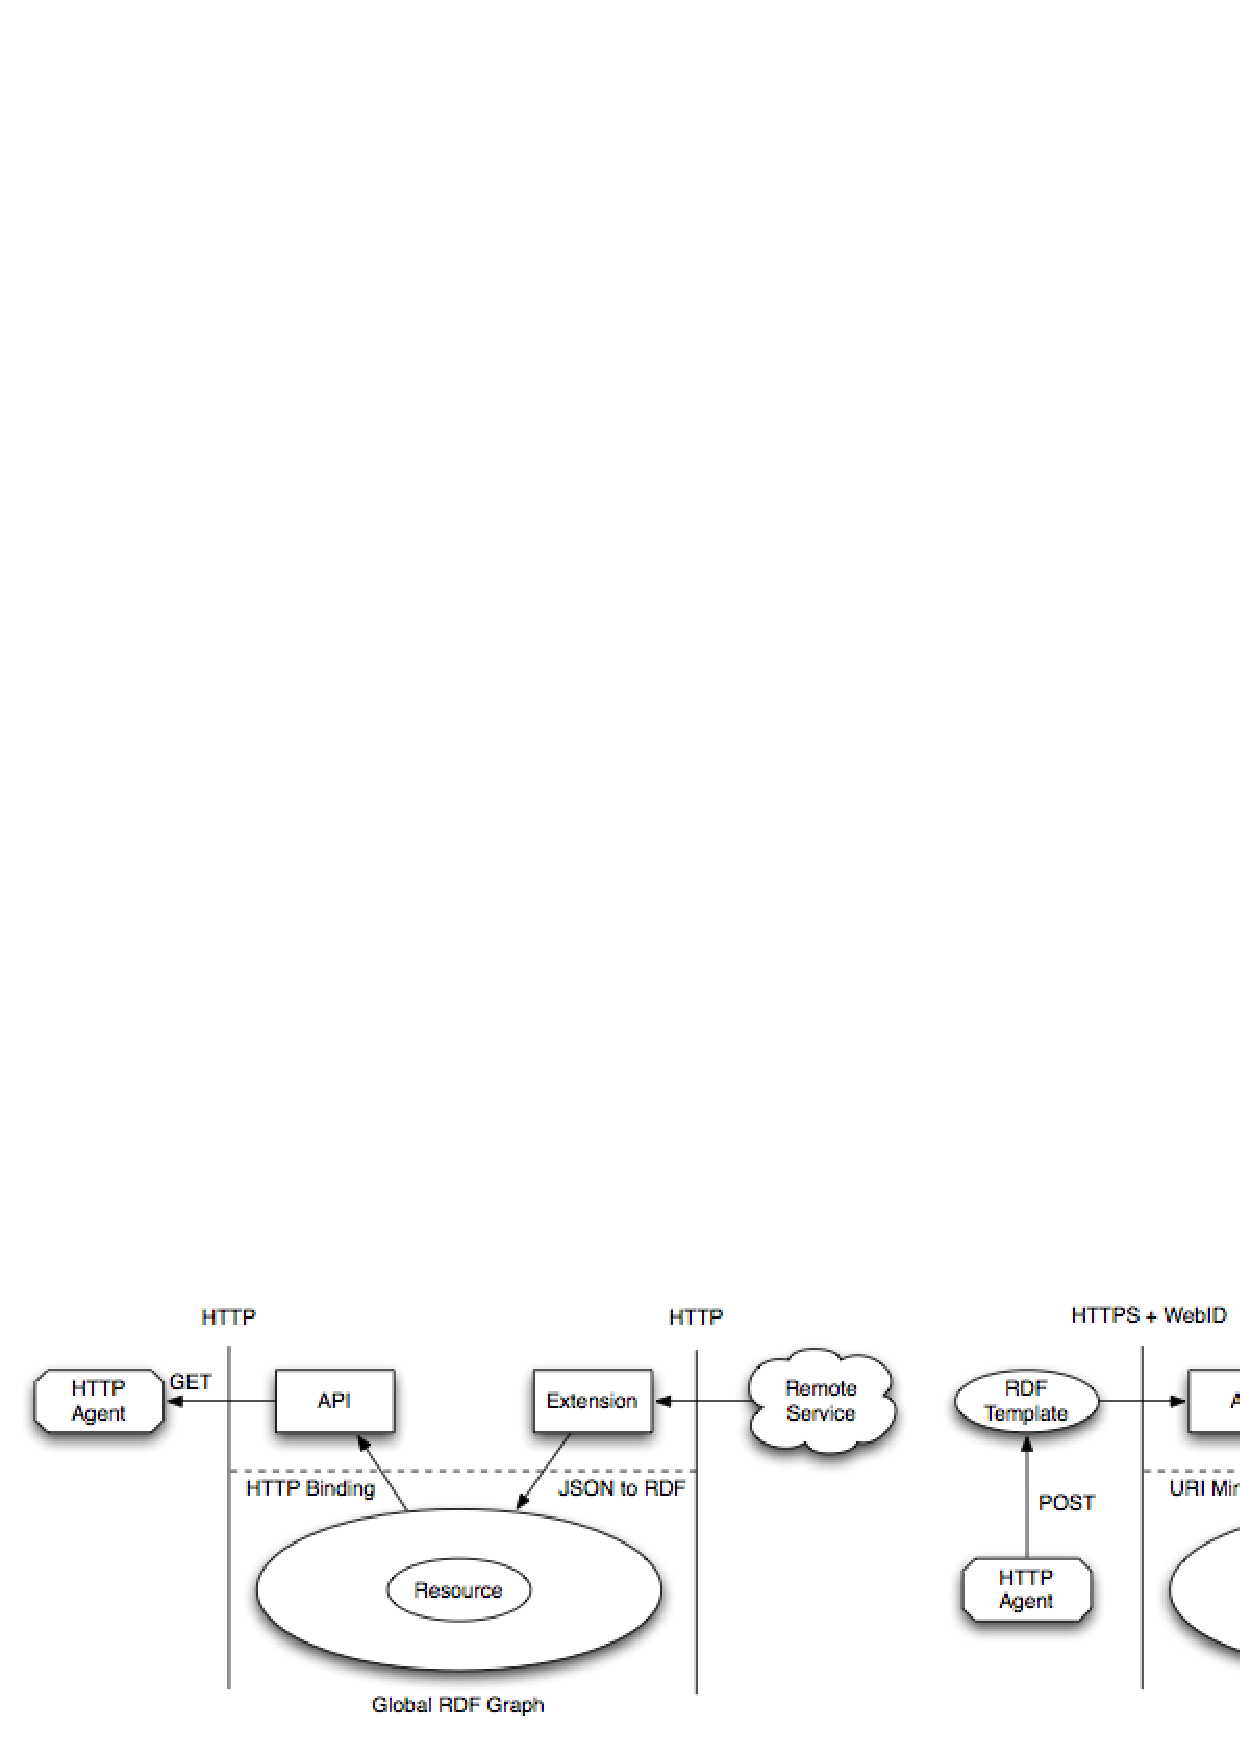
\includegraphics[width=0.5\textwidth]{figura5}
\label{figura5}
\end{figure}


\begin{itemize}
\item \textbf{Concepci\'on de la aplicaci\'on como un sistema modular.} Cada m\'odulo gestiona la interacci\'on con una red social diferente y se ejecutan de una forma completamente aut\'onoma cooperando a trav\'es del uso de un mecanismos de mensajes y de una ontolog\'ia \textit{RDF} com\'un donde se exponen los tipos de recursos que la extensi\'on va a generar. Gracias a este vocabulario com\'un, el n\'ucleo com\'un de la aplicaci\'on es capaz de integrar esos recurso en la \textit{API} \textit{HTTP}, recuperarlos del repositorio \textit{RDF} y darles el formato adecuado si es necesario.
\item \textbf{Integraci\'on de la autenticaci\'on \textit{WebID}.} En la definici\'on de la arquitectura de servicios \textit{REST} sem\'anticos expuesta anteriormente no se mencionaron los aspectos de seguridad relativas a la autenticaci\'on del acceso a los recursos expuestos. La aplicaci\'on construida soluciona este problema mediante el uso de \textit{WebID}. Cualquier recurso expuesto a trav\'es de la \textit{API} o tipo de recursos, puede ser marcado como publico, privado o accesible s\'olo por un determinado n\'umero de identidades \textit{WebID}. El sistema se encarga de autenticar la identidad de los usuarios accediendo a los recurso en cada petici\'on \textit{HTTP} realizando el proceso de autenticaci\'on \textit{WebID} y comprobando el grafo \textit{RDF} resultante de a\~nadir la informaci\'on de perfil remoto obtenida con los datos de perfil de usuario mantenidos localmente. Este proceso es completamente \textit{REST} involucrando simplemente la desrefernciaci\'on de la \textit{URI} asociada a la identidad del cliente y la verificaci\'on criptogr\'afica de su validez.
\item \textbf{Exposici\'on de un flujo social de datos.} El concepto de flujo social se traduce mal en t\'erminos \textit{REST} tanto por su naturaleza no discreta y din\'amica, como por el hecho de estar pensado para ser consumido mediante un mecanismo \textit{push} en el que el servicio notifica a los clientes de la presencia de nuevos datos. En nuestra implementaci\'on hemos optado por una opci\'on intermedia en el que el consumo del flujo es todav\'ia \textit{pull} siendo los clientes los encargados de realizar alg\'un tipo de petici\'on peri\'odica para obtener los nuevos eventos expuestos. Para ello, el flujo se asocia a una \textit{URI} estable y bien conocida, donde los clientes pueden realizar peticiones de solo lectura mediante operaciones \textit{GET} \textit{HTTP}. Las diferentes extensiones aut\'onomas de la aplicaci\'on pueden publicar en cualquier momento informaci\'on en el flujo insertando en el grafo recursos \textit{RDF} con un tipo \textit{SIOC} \textit{MicroBlogPost}.
\item \textbf{Implementaci\'on de \textit{SPARQL} WebHooks}. Para mitigar el problema del consumo del flujo de datos mediante peticiones peri\'odicas, el sistema tambi\'en emplea un sistema que permite a un cliente con una \textit{URI} desreferenciable e identificado por una identidad \textit{WebID} crear una petici\'on de notificaci\'on web (\textit{WebHook}) con una consulta \textit{SPARQL} asociada. Si una modificaci\'on del grafo de la aplicaci\'on resulta en una respuesta satisfactoria de la consulta \textit{SPARQL}, los resultados ser\'an enviadas a la \textit{URI} provista por la identidad \textit{WebID} que creo la petici\'on de notificaci\'on en el sistema. Las peticiones de notificaci\'on se exponen en el sistema como otro recurso sem\'antico m\'as con la excepci\'on de que puedenser manipuladas, no solo por el administrador del servicio, sino por los clientes remotos que crearon dicas peticiones de notificaci\'on.
\end{itemize}

\subsubsection{Detalles de implementaci\'on}

El prototipo del sistema aqu\'i detallado fue implementado usando la plataforma de desarrollo de aplicaciones \textit{JavaScript} \textit{Node.JS}. La capa de persistencia \textit{RDF} se implement\'o usando la base de datos no relacional MongoDB, donde se almacenaron las \textit{mol\'ecula}s \textit{RDF} directamente como objetos \textit{JSON-LD}. Los componentes para llevar a cabo la generaci\'on de identidades \textit{WebID} o llevar a cabo la autenticaci\'on tambi\'en fueron desarrollados como bibliotecas para \textit{Node.JS} y liberados posteriormente con licencia de C\'odigo Abierto.\\
En aquellos momentos en el que la ejecuci\'on de consultas \textit{SPARQL} resultaba indispensable, nuestra librer\'ia implementado un repositorio \textit{RDF} \textit{JavaScript} con soporte para \textit{SPARQL 1.1 Update} fue utilizada, cargando en el repositorio los documentos \textit{JSON-LD} recuperados desde MongoDB que son necesarios.
Como parte de la implementaci\'on del sistema, componentes modulares para los servicios de web sociales Twitter, Github y un componente gen\'erico para feeds RSS/Atom fueron desarrollados.\\
La \textit{API} \textit{HTTP} expuesta soporta peticiones procedentes de clientes \textit{JavaScript} ejecut\'andose en browser desde dominios diferentes a los del servicio gracias a la implementaci\'on del est\'andar de peticiones \textit{cross domain} (\textit{CORS}) \cite{cors} de la \textit{W3C}.\\
Por \'ultimo, algunas aplicaciones clientes \textit{JavaScript} han sido desarrollados e incluidas en el sistema para consumir la \textit{API} que el servicio expone. Una primera aplicaci\'on administrativa accede a los recursos de perfil y configuraci\'on de la \textit{API} para configurar la informaci\'on de perfil del usuario del servicio as\'i, como las pol\'iticas de acceso a los recursos expuestos y de gesti\'on de la identidad \textit{WebID} del usuario.\\
La figura \ref{figura6} muestra el aspecto de otra de las aplicaciones incluidas capaz de visualizar el flujo social de una identidad \textit{WebID} alojada en el servicio. Se puede observar como notificaciones generadas por diferentes componentes (Twitter, Github) se mezclan en el flujo social del usuario. \\

\begin{figure}
\vspace{2.4in}
\caption{Aplicaci\'on \textit{JavaScript} mostrando el flujo de actividad de un usuario.}
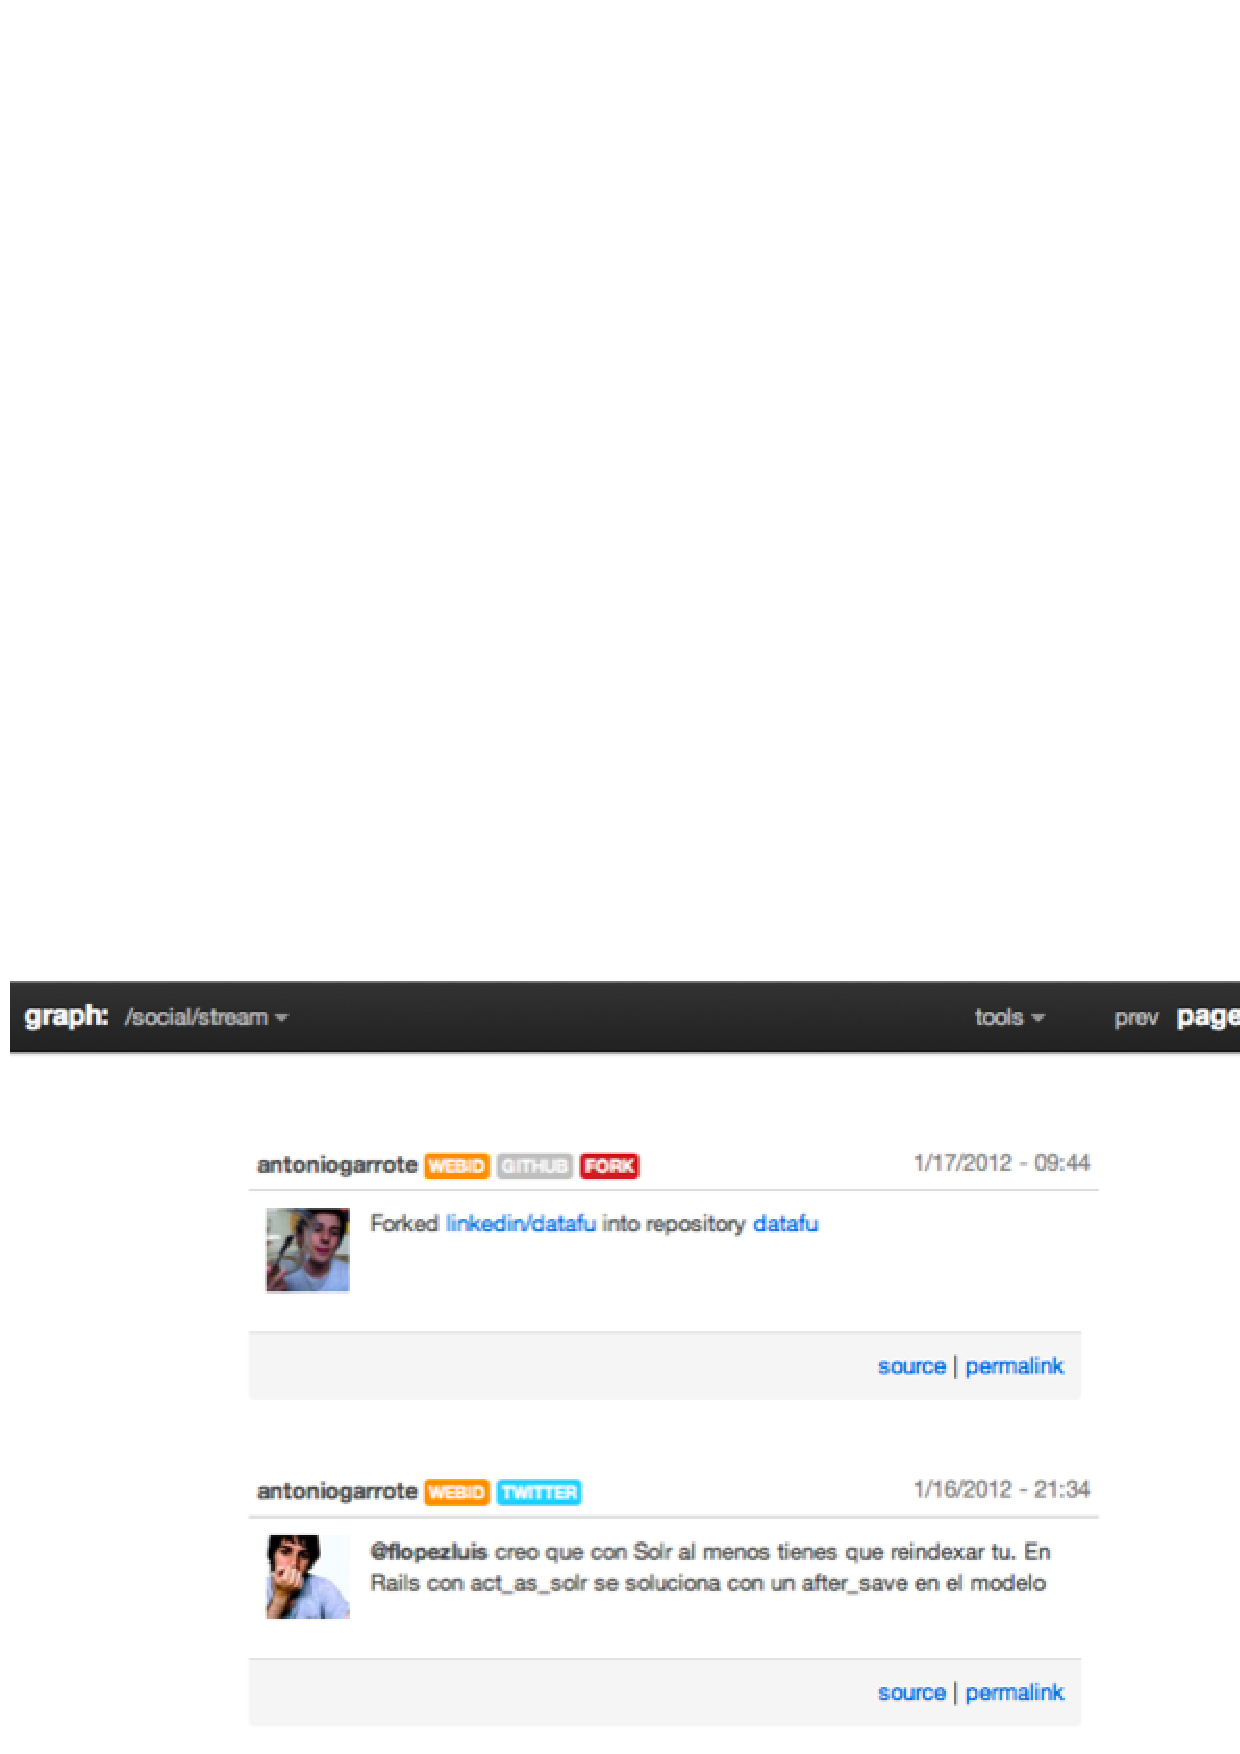
\includegraphics[width=0.5\textwidth]{figura6}
\label{figura6}
\end{figure}


Ambas aplicaciones usan nuestro repositorio \textit{RDF} \textit{JavaScript} ejecut\'andose en el navegador para agregar los recursos \textit{REST} sem\'anticos expuestos a trav\'es de la \textit{API} de datos enlazados sem\'anticos y construir con ellos una p\'agina final \textit{HTML} que tambi\'en incorpora la informaci\'on \textit{RDF} extra\'ida mediante el uso del est\'andar \textit{RDFa}.

\subsection{Visualizaci\'on de datos \textit{RDF} en aplicaciones \textit{JavaScript}}

En el caso de aplicaci\'on anterior, hemos visto como el uso de una \textit{API} de datos enlazados sem\'anticos hace posible transformar el dise\~no y las caracter\'isticas de un dominio de aplicaci\'on especifico, como es el caso de la construcci\'on de redes sociales de usuarios. En esta secci\'on nos centraremos en un caso de aplicaci\'on m\'as concreto, como es el de la construcci\'on de visualizaciones de datos en un cliente \textit{JavaScript} ejecut\'andose en el navegador, para intentar mostrar como el uso de informaci\'on sem\'antica disponible en una \textit{API} enlazada sem\'antica y el uso de librer\'ias espec\'ificas que hagan su tratamiento sencillo, como el repositorio \textit{RDF} \textit{JavaScript} que hemos descrito en secciones anteriores, permite ofrecer soluciones alternativas m\'as simples en este dominio de aplicaci\'on.\\
Generar visualizaciones de datos a partir de grafos \textit{RDF}, especialmente usando \textit{JavaScript} en el navegador es un proceso complejo y tedioso. La dificultad radica en el hecho de que las bibliotecas de visualizaci\'on de datos disponibles, como \textit{D3} \cite{d3}, no est\'an preparadas para trabajar directamente con el modelo de datos \textit{RDF}, necesit\'andose por tanto, un proceso de limpieza y transformaci\'on de los datos en el modelo de datos que la biblioteca demanda para cada tipo de visualizaci\'on en concreto.\\
En esta secci\'on describiremos una biblioteca \textit{JavaScript} para la construcci\'on de visualizaciones de datos, que tiene en cuenta las caracter\'isticas del modelo de datos \textit{RDF} para definir la visualizaci\'on. El sistema se ha construido sobre la biblioteca que implementa un repositorio \textit{RDF} para \textit{JavaScript} con soporte para consultas \textit{SPARQL 1.1 Update} que describimos en secciones anteriores.

\subsubsection{Gram\'atica de gr\'aficos para \textit{RDF}}

La biblioteca se ha construido sobre las ideas de una gram\'atica de gr\'aficos \cite{wilkinson2012grammar}, un conjunto finito de operaciones de alto nivel que se pueden combinar de diferentes maneras para generar un numero determinado visualizaciones gr\'aficas, dados unos datos iniciales de entrada.\\
La biblioteca construida extiende las operaciones cl\'asicas de este tipo de gram\'aticas de gr\'aficos,  con dos operaciones espec\'ificas para manipular datos \textit{RDF}:

\begin{itemize}
\item \textbf{Selecci\'on de datos \textit{RDF}}, mediante consultas \textit{SPARQL} y la selecci\'on de una estructura de datos de destino: lista, \'arbol o grafo, donde los nodos \textit{RDF} seleccionados ser\'an autom\'aticamente coercionados.
\item \textbf{\textit{Join} de datos generalizado}. Mediante el cual los nodos \textit{RDF} recuperados e introducidos en la estructura de datos seleccionada, son asociados a marcas visuales en la visualizaci\'on, traduci\'endose durante el proceso las propiedades \textit{RDF} del recurso en caracter\'isticas visuales de la marca visual asociada, como la posici\'on, el radio, la altura y anchura, el color, etc.
\end{itemize}

La tabla \ref{tabla13} muestra la sintaxis final de la biblioteca, mostrando como el vocabulario de la gram\'atica puede usarse para construir una visualizaci\'on. La figura \ref{figura7} muestra el resultado final de esa misma descripci\'on.\\

\begin{table}
\vspace{2.4in}
\caption{Definici\'on de una visualizaci\'on usando la gram\'atica de gr\'aficos.}
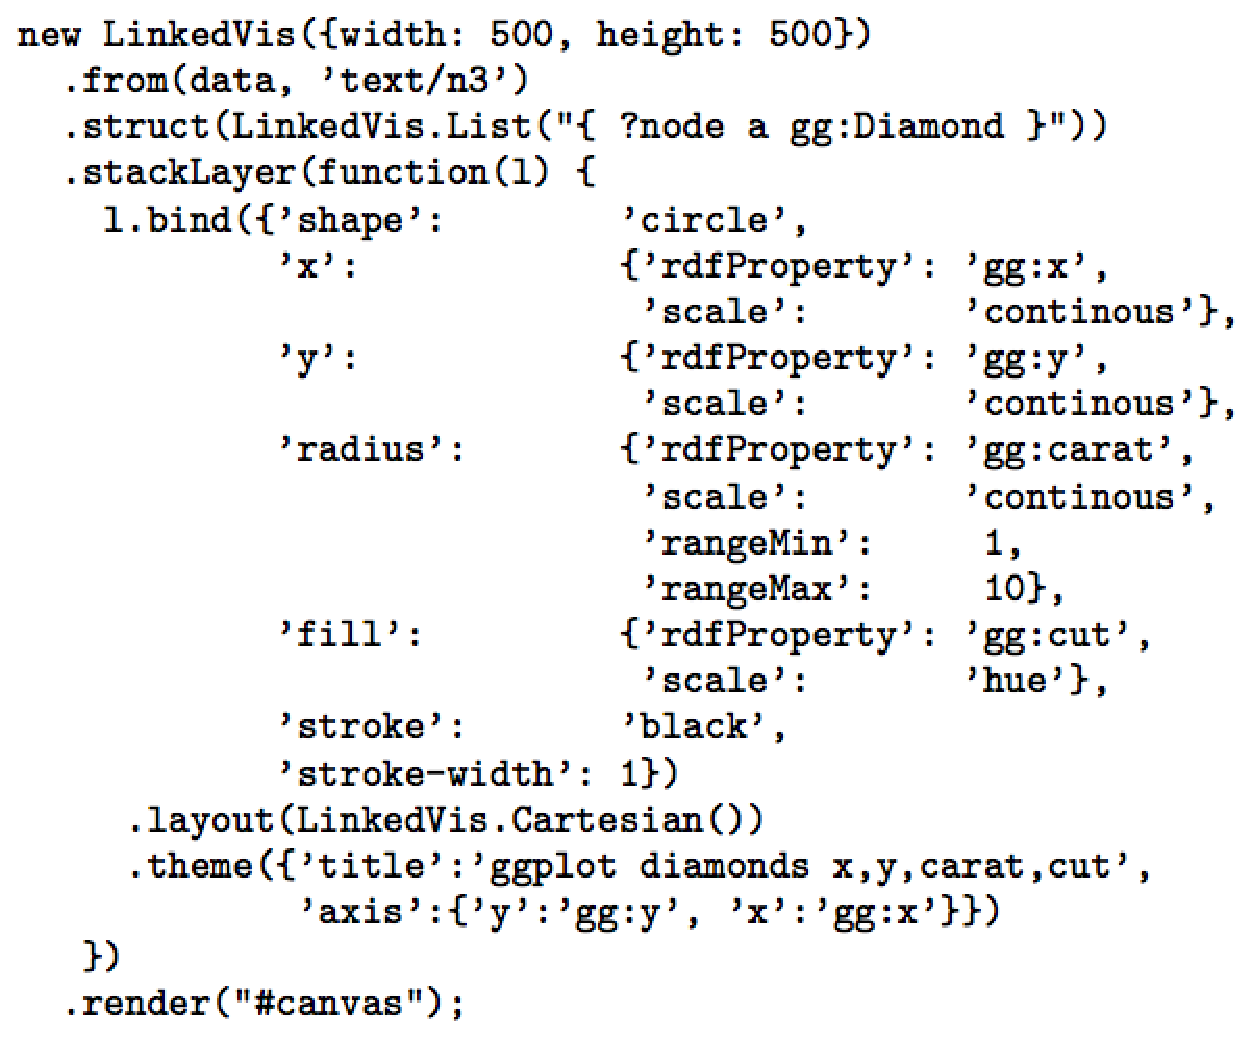
\includegraphics[width=0.8\textwidth]{tabla13}
\label{tabla13}
\end{table}

\begin{figure}
\vspace{2.4in}
\caption{Visualizaci\'on generada por la biblioteca a partir del c\'odigo de la tabla \ref{tabla13}}
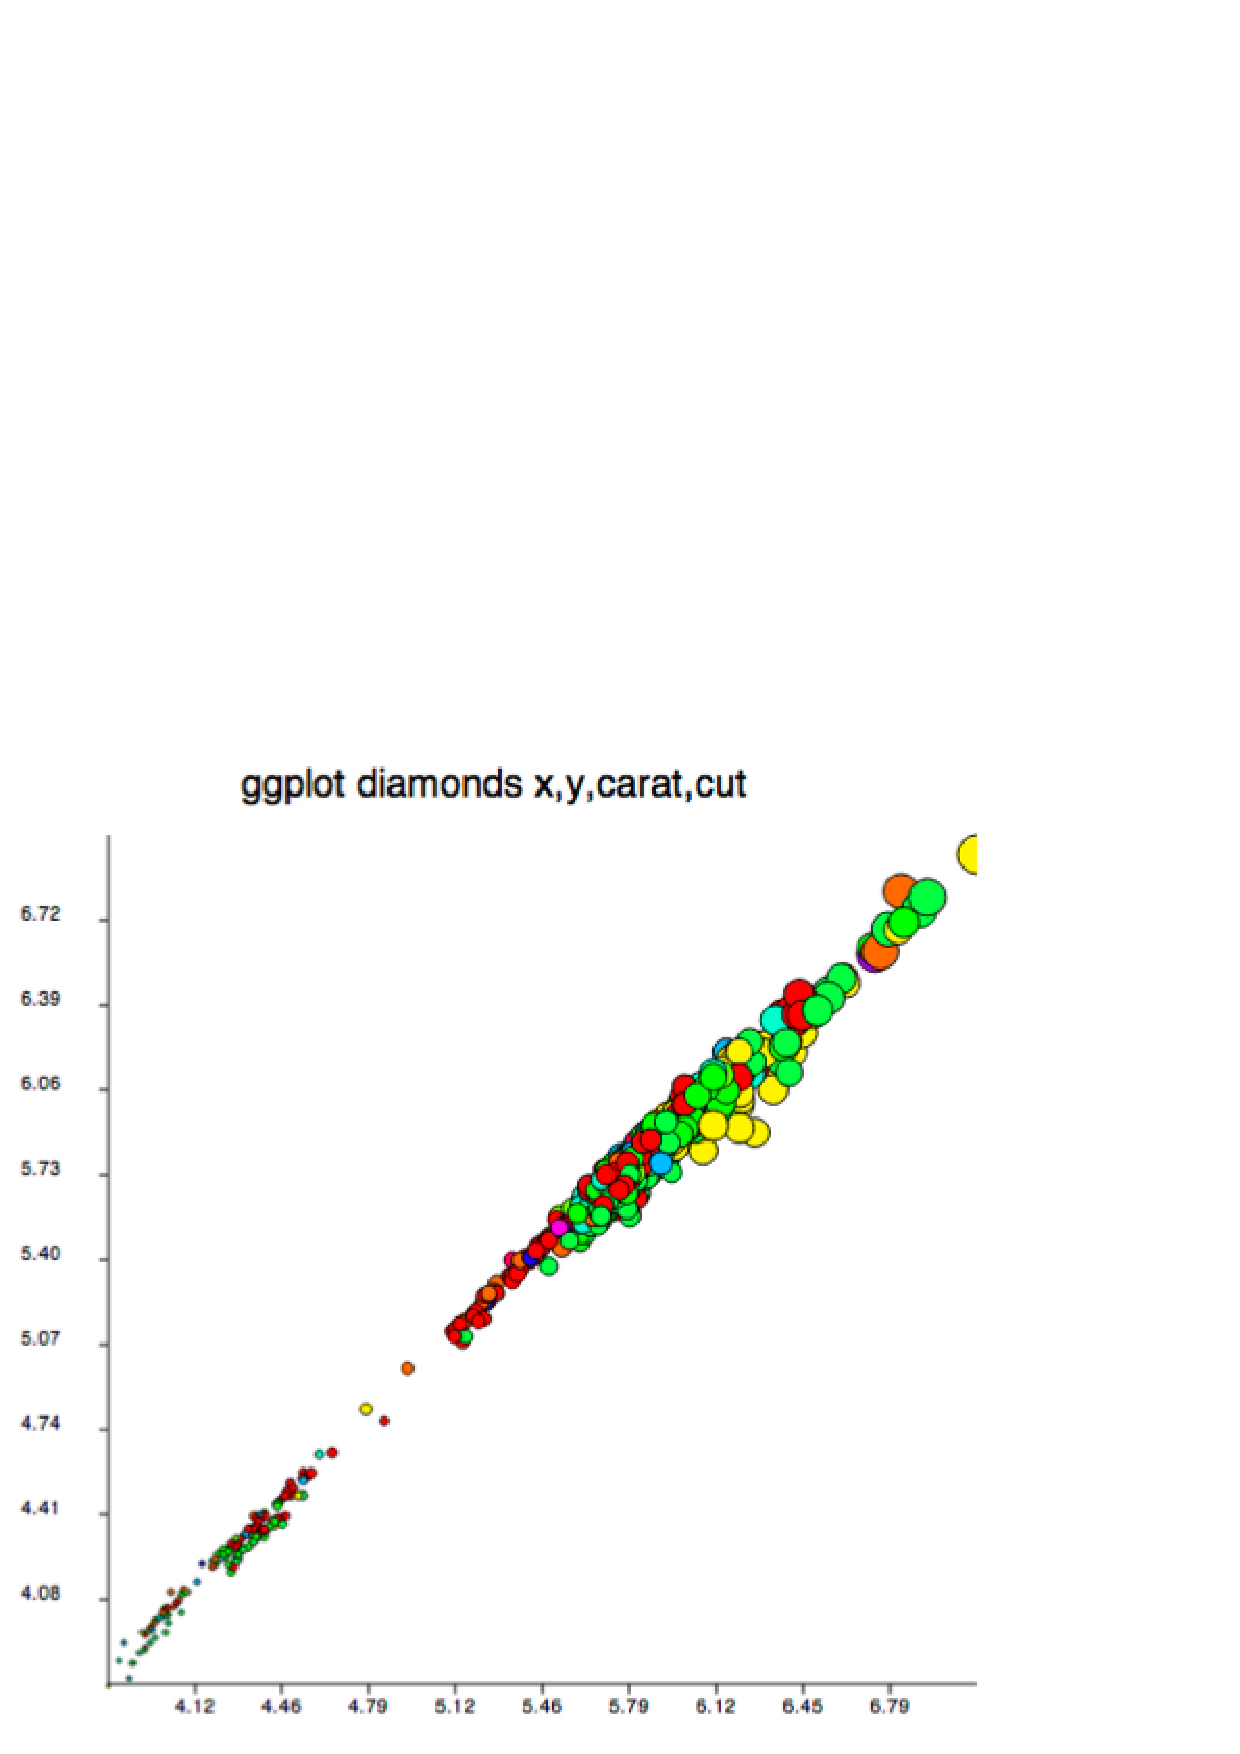
\includegraphics[width=0.5\textwidth]{figura7}
\label{figura7}
\end{figure}

Se puede observar como la funci\'on \textit{struct} introduce una estructura de datos de destino para los nodos \textit{RDF} recuperados por una consulta \textit{SPARQL}. A su vez, la funci\'on \textit{bind} realiza el \textit{join} entre datos y marcas visuales, usando para ello las propiedades \textit{RDF} de los nodos recuperados que son asignadas a diferentes valores de las propiedades de la marca.

\subsubsection{Dise\~no e implementaci\'on}

El dise\~no de la biblioteca se basa en la ejecuci\'on de cuatro etapas que conducen a la generaci\'on de la visualizaci\'on final como un documento \textit{SVG} insertado en el \'arbol \textit{DOM} de la p\'agina \textit{HTML} de destino.

\begin{itemize}
\item \textbf{Selecci\'on de datos}. Es el proceso por el que el usuario de la gram\'atica selecciona el origen de los datos \textit{RDF}, un recurso \textit{REST} sem\'antico remoto, el texto de un documento \textit{RDF} o una instancia del objeto repositorio \textit{RDF}, y lo transforma en una estructura de destina mediante una consulta \textit{SPARQL}. La biblioteca soporta tres diferentes estructuras de datos de desitno, listas, \'arboles y grafos. Cada una de estas estructuras requieren que el usuario especifique consultas \textit{SPARQL} con cierta estructura, usando valores espec\'ificos de las variables \textit{SPARQL} que luego ser\'an utilizados por la l\'ogica de la estructura de datos de destino para recuperar los datos.
\item \textbf{Composici\'on de capas}. La visualizaci\'on es construida por la biblioteca como un conjunto de capas que pueden ser superpuestas, compartiendo entonces los mismos l\'imites que la capa inferior,  o anidadas dentro de otra, con lo que la nueva capa queda restringida a un subarea de la capa padre. La capa recibe la selecci\'on de datos actual que ser\'a usada para generar las marcas visuales necesarias dentro de la capa.
\item \textbf{\textit{join} de marcas visuales}. Dentro de una capa, es posible realizar una operaci\'on de \textit{join} entre  los datos de la selecci\'on anterior y un tipo de marca visual con determinadas propiedades est\'eticas. La biblioteca soporta diferentes tipos de marcas, entre las que algunas coinciden con elementos \textit{SVG}, como \textit{rect}, \textit{circle} o \textit{text}. Las propiedades est\'eticas de cada marca se asocian a las propiedades \textit{RDF} del nodo \textit{RDF} que ha sido asignado a la marca mediante la operaci\'on de \textit{join}. Las propiedades est\'eticas se pueden clasificar en propiedades dimensi\'on, como la posici\'on \textit{x}, \textit{y}, el radio, etc, propiedades de estilo, modeladas de acuerdo a las propiedades \textit{CSS} como el color de relleno o el color de trazo y por \'ultimo, propiedades espec\'ificas para el tipo de layout que se ha asignado a la capa, como veremos a continuaci\'on. Los valores de estas propiedades est\'eticas se pueden especificar como un valor constante, el valor de la propiedad \textit{RDF} asociada o una funci\'on de escala que toma como valor de entrada el valor de la propiedad \textit{RDF}.
\item \textbf{Procesamiento del layout}. Cada capa de la visualizaci\'on debe declarar una propiedad de layout, usada por la biblioteca para computar la posici\'on de cada marca visual en la visualizaci\'on. Para ello el \textit{layout} utilizar\'a el valor de las propiedades est\'eticas de cada marca visual. Los \textit{layouts} soportados por la biblioteca se organizan de forma jer\'arquica, siendo los layouts cartesiano y polar los m\'as gen\'ericos. Distintos \textit{layouts} generan diferentes visualizaciones y exigen diferentes propiedades en las marcas visuales.
\end{itemize}

\subsubsection{Visualizaciones enlazadas}

Una de las funcionalidades de la biblioteca construida que no suele estar presente en otras soluciones para la generaci\'on de visualizaciones de datos es el de la inclusi\'on de abundantes meta-datos \textit{RDF} en la propia visualizaci\'on. Estos es posible gracias a que el formato \'ultimo de la visualizaci\'on generada consiste en un documento SVG con formato \textit{XML}. Dos grafos est\'an presentes en la visualizaci\'on final generada.

\begin{itemize}
\item \textbf{Grafo de datos}. Es un grafo \textit{RDF} conteniendo la agregaci\'on de todos los nodos \textit{RDF} seleccionados en todas las capas de la visualizaci\'on.
\item \textbf{Meta-grafo}. Conteniendo una descripci\'on de la visualizaci\'on usando una ontolog\'ia espec\'ifica. Este grafo incluye detalles como el n\'umero de capas, las estructuras de datos usadas o qu\'e nodos del grafo de datos est\'an asociados a qu\'e marcas visuales.
\end{itemize}

La presencia de ambos tipos de grafos abre la puerta a la construcci\'on de bibliotecas capaz de manipular la visualizaci\'on en funci\'on de la descripci\'on de la misma que se encuentra insertada en ella para a\~nadir un elemento de interactividad al uso que de la visualizaci\'on har\'an los usuarios finales. La generaci\'on de ambos grafos de meta-datos es opcional y puede ser desactivada.